\documentclass[12pt,twoside]{book}

\usepackage{mathptm,times,color}
\usepackage[pdftex]{graphicx}
\usepackage{multirow}
\usepackage{bezier}
\usepackage{rotating}
\usepackage{longtable}
\usepackage{amsmath}
\usepackage{xfrac}
\usepackage{array}
\usepackage{units}
\usepackage{fix-cm}
\usepackage{xspace}
\usepackage{makeidx} % Create index at end of document
\usepackage[nottoc,notlof,notlot]{tocbibind} % Put the bibliography and index in the ToC
\usepackage{datetime}
\newdateformat{mydate}{\monthname[\THEMONTH] \THEYEAR}

\usepackage{listings}
\usepackage{textcomp}
\definecolor{lbcolor}{rgb}{0.96,0.96,0.96}
\lstset{
    %backgroundcolor=\color{lbcolor},
    tabsize=4,
    rulecolor=,
    language=Fortran,
        basicstyle=\footnotesize\ttfamily,
        upquote=true,
        aboveskip={\baselineskip},
        belowskip={\baselineskip},
        columns=fixed,
        extendedchars=true,
        breaklines=true,
        breakatwhitespace=true,
        frame=none,
        showtabs=false,
        showspaces=false,
        showstringspaces=false,
        identifierstyle=\ttfamily,
        keywordstyle=\color[rgb]{0,0,0},
        commentstyle=\color[rgb]{0,0,0},
        stringstyle=\color[rgb]{0,0,0},
}

\usepackage{wrapfig}
\usepackage{morefloats}

\newcolumntype{L}[1]{>{\raggedright\let\newline\\\arraybackslash\hspace{0pt}}m{#1}}
\newcolumntype{C}[1]{>{\centering\let\newline\\\arraybackslash\hspace{0pt}}m{#1}}
\newcolumntype{R}[1]{>{\raggedleft\let\newline\\\arraybackslash\hspace{0pt}}m{#1}}

\IfFileExists{../Bibliography/gitrevision.tex}
{\input{../Bibliography/gitrevision}}
{\newcommand{\gitrevision}{unknown} }

\usepackage{framed}
\newcommand{\graybox}[1]{
\begin{shaded}#1\end{shaded}
}

\usepackage{changepage}

\renewcommand{\bibname}{References}

% dummy change to force revision update

%\usepackage{eso-pic}
%\usepackage{graphicx}
%\usepackage{color}
%\usepackage{type1cm}


%\makeatletter
%   \AddToShipoutPicture{%
%     \setlength{\@tempdimb}{.5\paperwidth}%
%    \setlength{\@tempdimc}{.5\paperheight}%
%   \setlength{\unitlength}{1pt}%
%  \put(\strip@pt\@tempdimb,\strip@pt\@tempdimc){%
%     \makebox(0,0){\rotatebox{45}{\textcolor[gray]{0.75}{\fontsize{8cm}{8cm}\selectfont{DRAFT}}}}}}
%\makeatother

\definecolor{linknavy}{rgb}{0,0,0.50196}
\definecolor{linkred}{rgb}{1,0,0}
\definecolor{linkblue}{rgb}{0,0,1}
\definecolor{shadecolor}{rgb}{0.9,0.9,0.9}

\usepackage[pdftex,
        colorlinks=true,
        urlcolor=linkblue,     % \href{...}{...} external (URL)
        citecolor=linkred,     % citation number colors
        linkcolor=linknavy,    % \ref{...} and \pageref{...}
        pdfproducer={pdflatex},
        pagebackref,
        pdfpagemode=UseNone,
        bookmarksopen=true,
        plainpages=false,
        verbose]{hyperref}

\usepackage{siunitx}
\sisetup{
    detect-all = true,
    input-decimal-markers = {.},
    input-ignore = {,},
    inter-unit-product = \ensuremath{{}\cdot{}},
    multi-part-units = repeat,
    number-unit-product = \text{~},
    per-mode = fraction,
    separate-uncertainty = true,
}

% CFAST Version String
\newcommand{\cfastversion}{7.2.3}

% commands to use for "official" cover and title pages
% see smokeview verification guide to see how they are used

\newcommand{\logosigs}{
\begin{minipage}[b]{6.5in}
\flushright{
\includegraphics[height=1.05in]{FIGURES/nistident}}
\end{minipage}
}

\newcommand{\titlesigs}
{
\small
\begin{flushright}
U.S. Department of Commerce \\
{\em Penny Pritzker, Secretary} \\
\hspace{1in} \\
National Institute of Standards and Technology \\
{\em Willie May, Acting Under Secretary of Commerce for Standards and Technology and Acting Director}
\end{flushright}
}

\newcommand{\headerA}[1]{
\begin{flushright}
\fontsize{20}{24}\selectfont
\bf{NIST Technical Note #1}
\end{flushright}
}


\newcommand{\headerB}[1]{
\begin{flushright}
\fontsize{28}{33.6}\selectfont
\bf{#1}
\end{flushright}
}

\newcommand{\headerC}[1]{
\vspace{.15in}
\begin{flushright}
\fontsize{12}{14}\selectfont
#1
\end{flushright}
}

\newcommand{\headerD}[1]{
\begin{flushright}
\fontsize{12}{14}\selectfont
This publication is available free of charge from: \\
http://dx.doi.org/10.6028/NIST.TN.#1
\end{flushright}
}

\newcommand{\coden}[1]{
\vspace*{\fill}
\begin{flushright}
\fontsize{12}{14}\selectfont
\textbf{National Institute of Standards and Technology Technical Note #1 \\
Natl. Inst. Stand. Technol. Tech. Note #1, \pageref{last_page} pages (\mydate\today) \\
CODEN: NTNOEF \\
\vspace{\baselineskip}
This publication is available free of charge from: \\
http://dx.doi.org/10.6028/NIST.TN.#1}
\end{flushright}
}



\setlength{\textwidth}{6.5in}
\setlength{\textheight}{9.0in}
\setlength{\topmargin}{0.in}
\setlength{\headheight}{0.in}
\setlength{\headsep}{0.in}
\setlength{\parindent}{0.25in}
\setlength{\oddsidemargin}{0.0in}
\setlength{\evensidemargin}{0.0in}

\newcommand{\vecy}{\mathbf{y}}
\newcommand{\vecF}{\mathbf{F}}
\newcommand{\rd}{\mathrm{d}}
\newcommand{\brackets}[1]{ { \left( {#1} \right) } }
\newcommand{\dcydt}[1]{\rd{#1}/\rd t}
\newcommand{\dbydt}[1]{\frac{\rd {#1}}{\rd t}}
\newcommand{\dbydx}[1]{\frac{\partial {#1}}{\partial x}}
\newcommand{\ddt}{\frac{\rd}{\rd t}}
\newcommand{\superscript}[1]{\ensuremath{^{\textnormal{\scriptsize \hbox{#1}}}}}
\newcommand{\subscript}[1]{\ensuremath{_{\textnormal{\scriptsize \hbox{#1}}}}}

\newcommand{\textct}[1]{\texttt{\small #1}}

\newcommand{\cp}{{\rm c}_{\rm p}}
\newcommand{\cv}{{\rm c}_{\rm v}}

\newcommand{\trho}{\tilde{\rho}}
\newcommand{\chia}{\chi_{\rm a}}
\newcommand{\chir}{\chi_{\rm r}}
\newcommand{\dph}{{\delta\phi}}
\newcommand{\dth}{{\delta\theta}}
\newcommand{\tp}{\tilde{p}}
\newcommand{\dQ}{\dot{Q}}
\newcommand{\dQc}{\dot{Q}_{\rm c}}
\newcommand{\dQr}{\dot{Q}_{\rm r}}
\newcommand{\Dh}{\Delta H}
\newcommand{\DhO}{\Delta H_\OTWO}
\newcommand{\Tp}{T_{\rm p}}
\newcommand{\Tu}{T_{\rm u}}
\newcommand{\Tl}{T_{\rm l}}
\newcommand{\Ti}{T_i}
\newcommand{\Tw}{\mathbf{T}_{\rm w}}
\newcommand{\Ts}{T_{\rm s}}
\newcommand{\Tg}{T_{\rm g}}
\newcommand{\TL}{T_{\rm L}}
\newcommand{\Vu}{V_{\rm u}}
\newcommand{\Vl}{V_{\rm l}}
\newcommand{\Vi}{V_i}
\newcommand{\doh}{\dot{h}}
\newcommand{\dhl}{\dot{h}_{\rm l}}
\newcommand{\dhu}{\dot{h}_{\rm u}}
\newcommand{\dmal}{\dot{m}_{\rm l}}
\newcommand{\dmau}{\dot{m}_{\rm u}}
\newcommand{\dq}{\dot{q}}
\newcommand{\dqc}{\dot{q}_{\rm c}}
\newcommand{\dqr}{\dot{q}_{\rm r}}
\newcommand{\dql}{\dot{q}_{\rm l}}
\newcommand{\dqu}{\dot{q}_{\rm u}}
\newcommand{\dqi}{\dot{q}_i}
\newcommand{\dm}{\dot{m}}
\newcommand{\dme}{\dot{m}_{\rm e}}
\newcommand{\dmp}{\dot{m}_{\rm p}}
\newcommand{\dml}{\dot{m}_{\rm l}}
\newcommand{\dmu}{\dot{m}_{\rm u}}
\newcommand{\dmi}{\dot{m}_i}
\newcommand{\dmf}{\dot{m}_{\rm f}}
\newcommand{\ml}{m_{\rm l}}
\newcommand{\mmu}{m_{\rm u}}
\newcommand{\mi}{m_i}

\newcommand{\be}{\begin{equation}}
\newcommand{\ee}{\end{equation}}

\newcommand{\RE}{\hbox{Re}}
\newcommand{\LE}{\hbox{Le}}
\newcommand{\PR}{\hbox{Pr}}
\newcommand{\PE}{\hbox{Pe}}
\newcommand{\NU}{\hbox{Nu}}
\newcommand{\SC}{\hbox{Sc}}
\newcommand{\SH}{\hbox{Sh}}
\newcommand{\WE}{\hbox{We}}

\newcommand{\COTWO}{{\tiny \hbox{CO}_2}}
\newcommand{\OTWO}{{\tiny \hbox{O}_2}}
\newcommand{\CO}{{\tiny \hbox{CO}}}
\newcommand{\HTWOO}{{\tiny \hbox{H}_2\hbox{O}}}
\newcommand{\NTWO}{{\tiny \hbox{N}_2}}
\newcommand{\F}{{\tiny \hbox{F}}}
\newcommand{\So}{{\tiny \hbox{S}}}
\newcommand{\M}{{\tiny \hbox{M}}}
\newcommand{\HCN}{{\tiny \hbox{HCN}}}
\newcommand{\HCl}{{\tiny \hbox{HCl}}}
\newcommand{\Hy}{{\tiny \hbox{H}}}
\newcommand{\C}{{\tiny \hbox{C}}}
\newcommand{\N}{{\tiny \hbox{N}}}
\newcommand{\Oh}{{\tiny \hbox{O}}}
\newcommand{\Cl}{{\tiny \hbox{Cl}}}

\newcommand{\asqh}{$A_T/A\sqrt{h}$}
\newcommand{\degc}{$^{\circ}$C\xspace}
\newcommand{\degf}{$^{\circ}$F\xspace}

\newcommand{\dx}{\delta x}
\newcommand{\dy}{\delta y}
\newcommand{\dz}{\delta z}
\newcommand{\dt}{\delta t}

\newcommand{\ha}{\frac{1}{2}}
\newcommand{\ft}{\frac{4}{3}}
\newcommand{\ot}{\frac{1}{3}}
\newcommand{\fofi}{\frac{4}{5}}
\newcommand{\of}{\frac{1}{4}}
\newcommand{\twth}{\frac{2}{3}}

\newcommand{\ct}{\tt\small}

\newcommand{\rb}[1]{\raisebox{1.5ex}[0pt]{#1}}

\newcommand{\erf}{\hbox{erf}}



\begin{document}

\bibliographystyle{unsrt}

\frontmatter

\pagestyle{empty}


\begin{minipage}[t][9in][s]{6.5in}

\headerA{1889v5\\}

\headerB{
CFAST -- Consolidated Fire \\
 and Smoke Transport \\
 (Version 7) \\
 Volume 5: CFAST Fire Data Generator (CData) \\
}

\headerC{
   Paul A. Reneke \\
   Richard D. Peacock \\
   Stanley W. Gilbert \\
   Thomas G. Cleary \\
}

\vfill

\headerD{1889v5}

\vfill

\logosigs

\end{minipage}

\newpage

\hspace{5in}

\newpage

\begin{minipage}[t][9in][s]{6.5in}

\headerA{1889v5\\}

\headerB{
CFAST -- Consolidated Fire \\
 And Smoke Transport \\
 (Version 7) \\
 Volume 5: CFAST Fire Data Generator (CData) \\
}

\headerC{
   Paul A. Reneke \\
   Richard D. Peacock \\
   Thomas G. Cleary \\

{\em Fire Research Division, Engineering Laboratory, Gaithersburg, Maryland} \\

Stanley W. Gilbert\\

{\em Office of Economics, Engeneering Laboratory, Gaithersburg, Maryland}\\
}

\headerD{1889v5}

\headerC{
\flushright{\mydate\today\\
CFAST Version \cfastversion \\
\emph{GIT Revision:}~\gitrevision}}

\vfill

\flushright{
\includegraphics[width=1.2in]{FIGURES/doc} }

\titlesigs

\end{minipage}


\newpage

\frontmatter

\pagestyle{plain}
\setcounter{page}{3}

%
% -------------------  Preface ------------------------
%

\chapter{Preface}

This document provides ...

%
% -------------------  Disclaimer ------------------------
%

\chapter{Disclaimer}

The US Department of Commerce makes no warranty, expressed or implied, to users of CFAST, and accepts no responsibility for its use. Users of CFAST assume sole responsibility under Federal law for determining the appropriateness of its use in any particular application; for any conclusions drawn from the results of its use; and for any actions taken or not taken as a result of analysis performed using these tools.

Users are warned that CFAST is intended for use only by those competent in the fields of fluid dynamics, thermodynamics, heat transfer, combustion, and fire science, and is intended only to supplement the informed judgment of the qualified user. The software package is a computer model that may or may not have predictive capability when applied to a specific set of factual circumstances. Lack of accurate predictions by the model could lead to erroneous conclusions with regard to fire safety. All results should be evaluated by an informed user.

Throughout this document, the mention of computer hardware or commercial software does not constitute endorsement by the National Institute of Standards and Technology, nor does it indicate that the products are necessarily those best suited for the intended purpose.

\coden{1889v5}

%
% -------------------  Acknowledgments ------------------------
%

\chapter{Acknowledgments}

\label{acksection}

CFAST was originally developed by Walter Jones, formerly of NIST.

Continuing support for CFAST is via internal funding at NIST. In addition, support is provided by other agencies of the U.S. Federal Government, most notably the Nuclear Regulatory Commission (NRC) and the Department of Energy (DOE). The NRC Office of Research has funded key validation experiments, the preparation of the CFAST manuals, and the continuing development of sub-models that are of importance in the area of nuclear power plant safety. Special thanks to Mark Salley and David Stroup for their support. Support to refine the software development and quality assurance process for CFAST has been provided by the DOE. The assistance of Subir Sen and Debra Sparkman is gratefully acknowledged.

\cleardoublepage
\tableofcontents

\clearpage
\listoffigures

\listoftables


\mainmatter

%
% -------------------  Introduction ------------------------
%

\chapter{Introduction}

The Monte Carlo method is "a broad class of computational algorithms that use repeated random sampling to obtain numerical results." with Stanislaw Ulam credited with inventing the modern version of the Markov Chain Monte Carlo method working on nuclear weapons projects in the 1940s. In the 80’s and before research was on going to make use of Monte Carlo idea as a part of the move toward performance-based designs in fire safety engineering. Bukowski \cite{Bukowski_1985}, Clarke et al. \cite{Clarke_1990}, and more recently, building codes \cite{NFPA_5000} and engineering handbooks \cite{Hurley_2016} provide a structure for a fire hazard analysis that can be used to characterize the relative performance of two sets of fire scenarios. Bruns \cite{bruns_tn_2016} formalized the mathematics for applying the Monte Carlo method to fire hazard analysis as a means to further incorporate the method in regular preformance based designs. However, one of the limiting factors in a more widespread adoption of Monte Carlo analysis has been the large amount of data that needs to be generated and processed.

While at one time the issue was one of both computational power and tools designed to do the analysis that is not as true anymore. With the inexorable power of Moore’s Law, it is now relatively easy to obtain the computational power and storage to generate and analysis huge amounts of data. What is still largely lacking are the tools to make the process tenable. To that end the Fire Research Division at the National Institute of Standards and Technology has been exploring the process \cite{NIST_TN_2041,Reneke_2017,Reneke_2018,Cleary_2019} in order to develop tools that will make Monte Carlo analysis a more widely used form of analysis. The result of this effort is the CFAST Fire Data Generator (CData).

%
% -------------------  Defining the Analysis ------------------------
%

\chapter{Defining the Question and the Analysis}

As briefly discussed in the introduction a significant amount of work has gone into understanding the basic requirements for a Monte Carlo analysis in a fire safety analysis [1,2]. They outline several key areas that need to be addressed in the analysis.  These include definition of:

\begin{enumerate}
  \item Community / Building / Occupant characteristics
  \item Fire scenarios
  \item Analysis variables / Criteria for comparisons
  \item Statistical analysis of calculation results
\end{enumerate}

Community, building, and fire characteristics define the physical geometries of the model simulations (the range of building geometries, vents between compartments and the outside, and the range of fires to be studied). Occupant characteristics and criteria for comparisons define additional model inputs that may be necessary for analysis of calculation results (fire detection devices, the choice of additional model outputs to study tenability of egress paths, fire severity, or building structural integrity, for example). All of these may be defined by a single deterministic set of inputs (a single building geometry or desired fire for study), a collection of different, specific inputs (such as a set of specific building designs of interest), or a statistically-determined range of inputs (for example, defining compartment sizes or smoke detector activation from experimentally-determined distributions). This section details the process for defining a series of input files for analysis with examples for each major step in the process.

\section{Building Characteristics}

In CFAST, compartment geometry includes definition of the number of compartments, their size (length, width, and height), and their placement in relation to other compartments. In the study of a single structure, this is simply an enumeration of each compartment. Figure \ref{sample_visualization} shows the compartments in a single structure in a CFAST simulation.

\begin{figure}[h!]
\centering
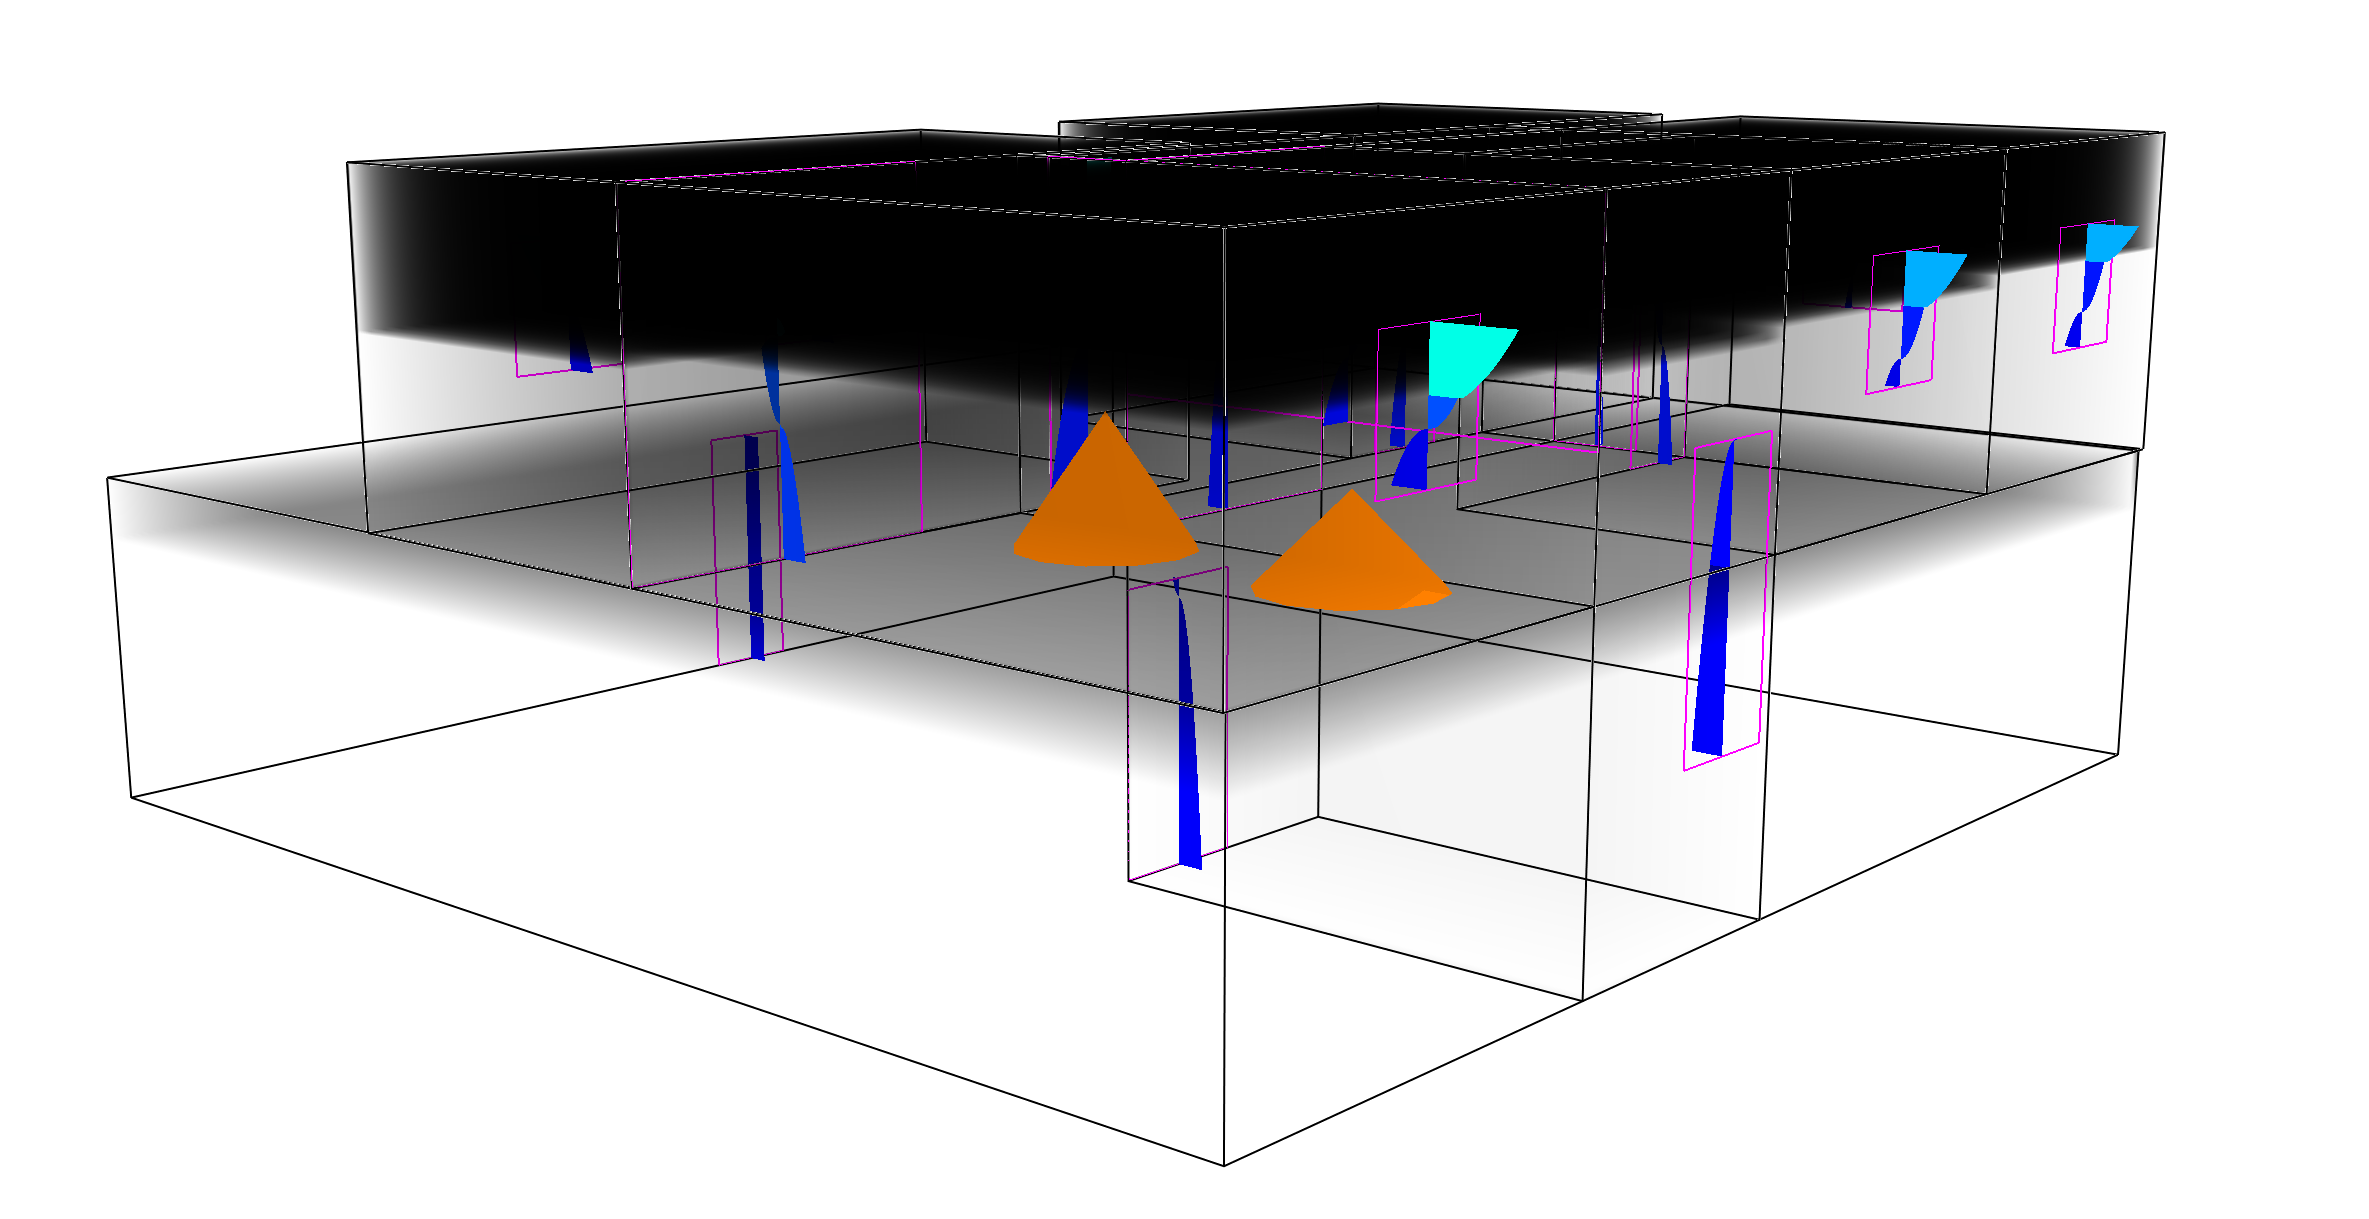
\includegraphics[width=4.5in]{FIGURES/Sample_Visualization.png}
\caption{Sample CFAST visualization of a single structure subject to a fire.}
\label{sample_visualization}
\end{figure}

Of course, if it is desired to study the impact of fires in a set of more than one specific building, the compartment geometry and placement could be defined by multiple individual buildings with the specific building chosen for an individual scenario chosen at random or from a distribution representing the population of each building type in the community under study.

The set of buildings for study can also be chosen from distributions of building and room characteristics. Figure \ref{sample_room_distribution} shows the distribution of the total floor area in a residence, the number of bedrooms in a residence depending on the total floor area, the total number of rooms given a certain number of bedrooms (here shown for residences from 1000~ft$^2$ to 1500~ft$^2$), all taken from the 2015 U.S. Housing Survey \cite{AHS2015}. Creating a compartment geometry from these data can be thought of as a six step process:

\begin{enumerate}
    \item randomly select the total floor area of the structure, Fig. \ref{sample_room_distribution}(a);
    \item randomly select the total number of bedrooms for a structure of the size chosen in step 1, Fig. \ref{sample_room_distribution}(b);
    \item randomly select the total number of rooms in the structure of the chosen size and number of bedrooms (Fig. \ref{sample_room_distribution}(c) shows a sample distribution for homes ranging from 1000~ft$^2$ to 1500~ft$^2$. Distributions for other home sizes are available in ref. \cite{AHS2015});
    \item determine room sizes based on a distribution of bedroom sizes, allocating left over space to the other rooms;
    \item connect compartments as desired (for example by randomly setting vents as open or closed between compartment pairs); and
    \item ensure that the resulting structure is realizable (This random approach to generating connections has a probability of resulting in a floorplan that cannot be instantiated in a single story. More technically, if the floorplan is thought of as a graph with the rooms as vertices and the connections as edges, some of the randomly generated graphs will be nonplanar for cases with more than four rooms. A planar graph is one that can be drawn on a piece of paper and none of the edges cross. The probability of generating a nonplanar floorplan increases as the number of rooms increases. In order to eliminate such nonphysical cases from the analysis, any randomly generated floorplan can be checked for planarity and rejected if necessary and replaced by a new randomly generated floorplan).
\end{enumerate}

\begin{figure}[p]
\begin{tabular*}{\textwidth}{c}
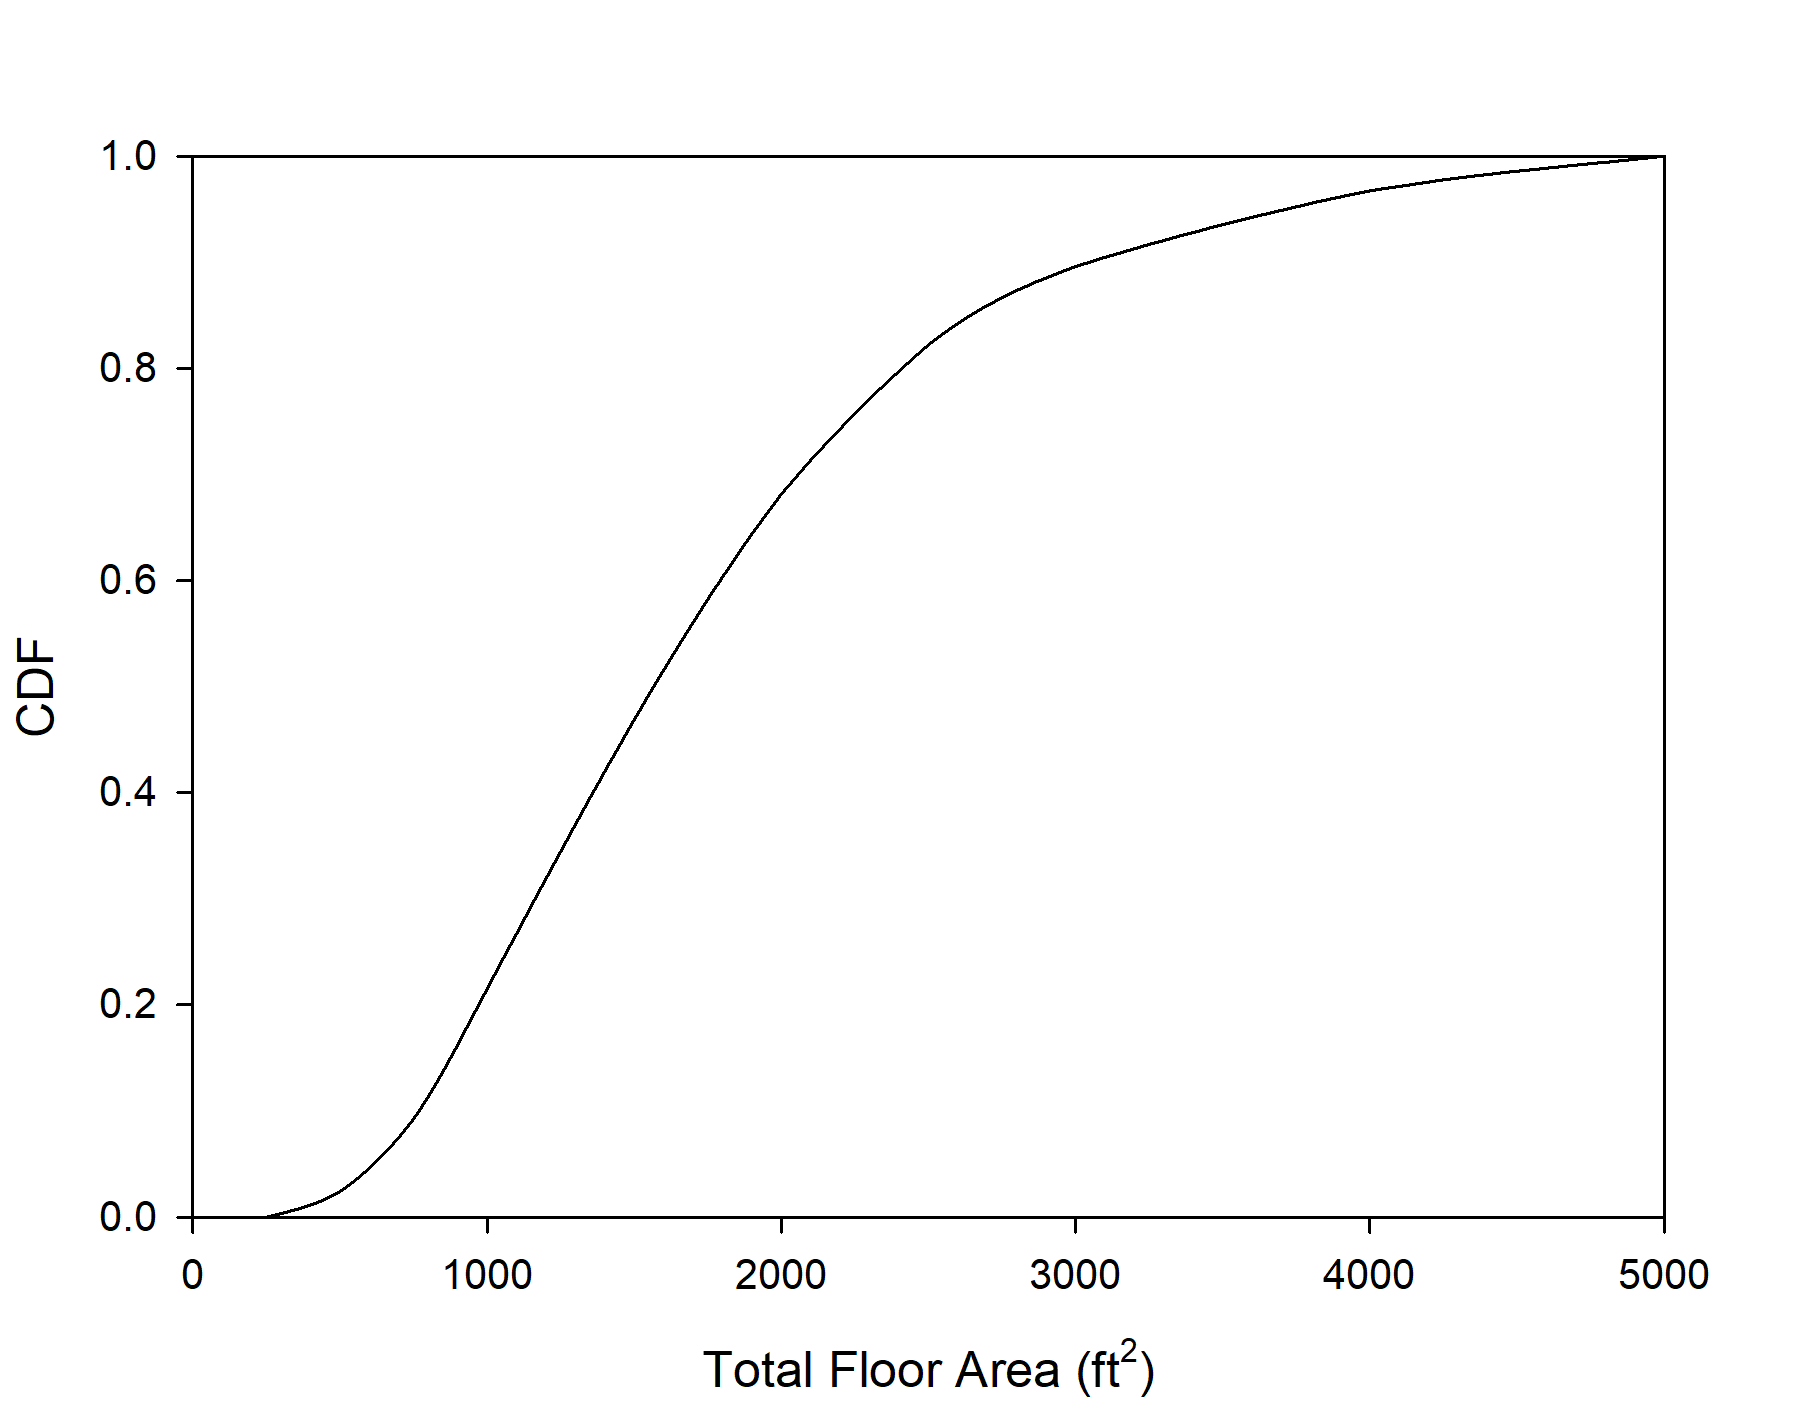
\includegraphics[height=2.5in]{FIGURES/Total_Floor_Area} \\
(a) Total Floor Area in a Residence \\
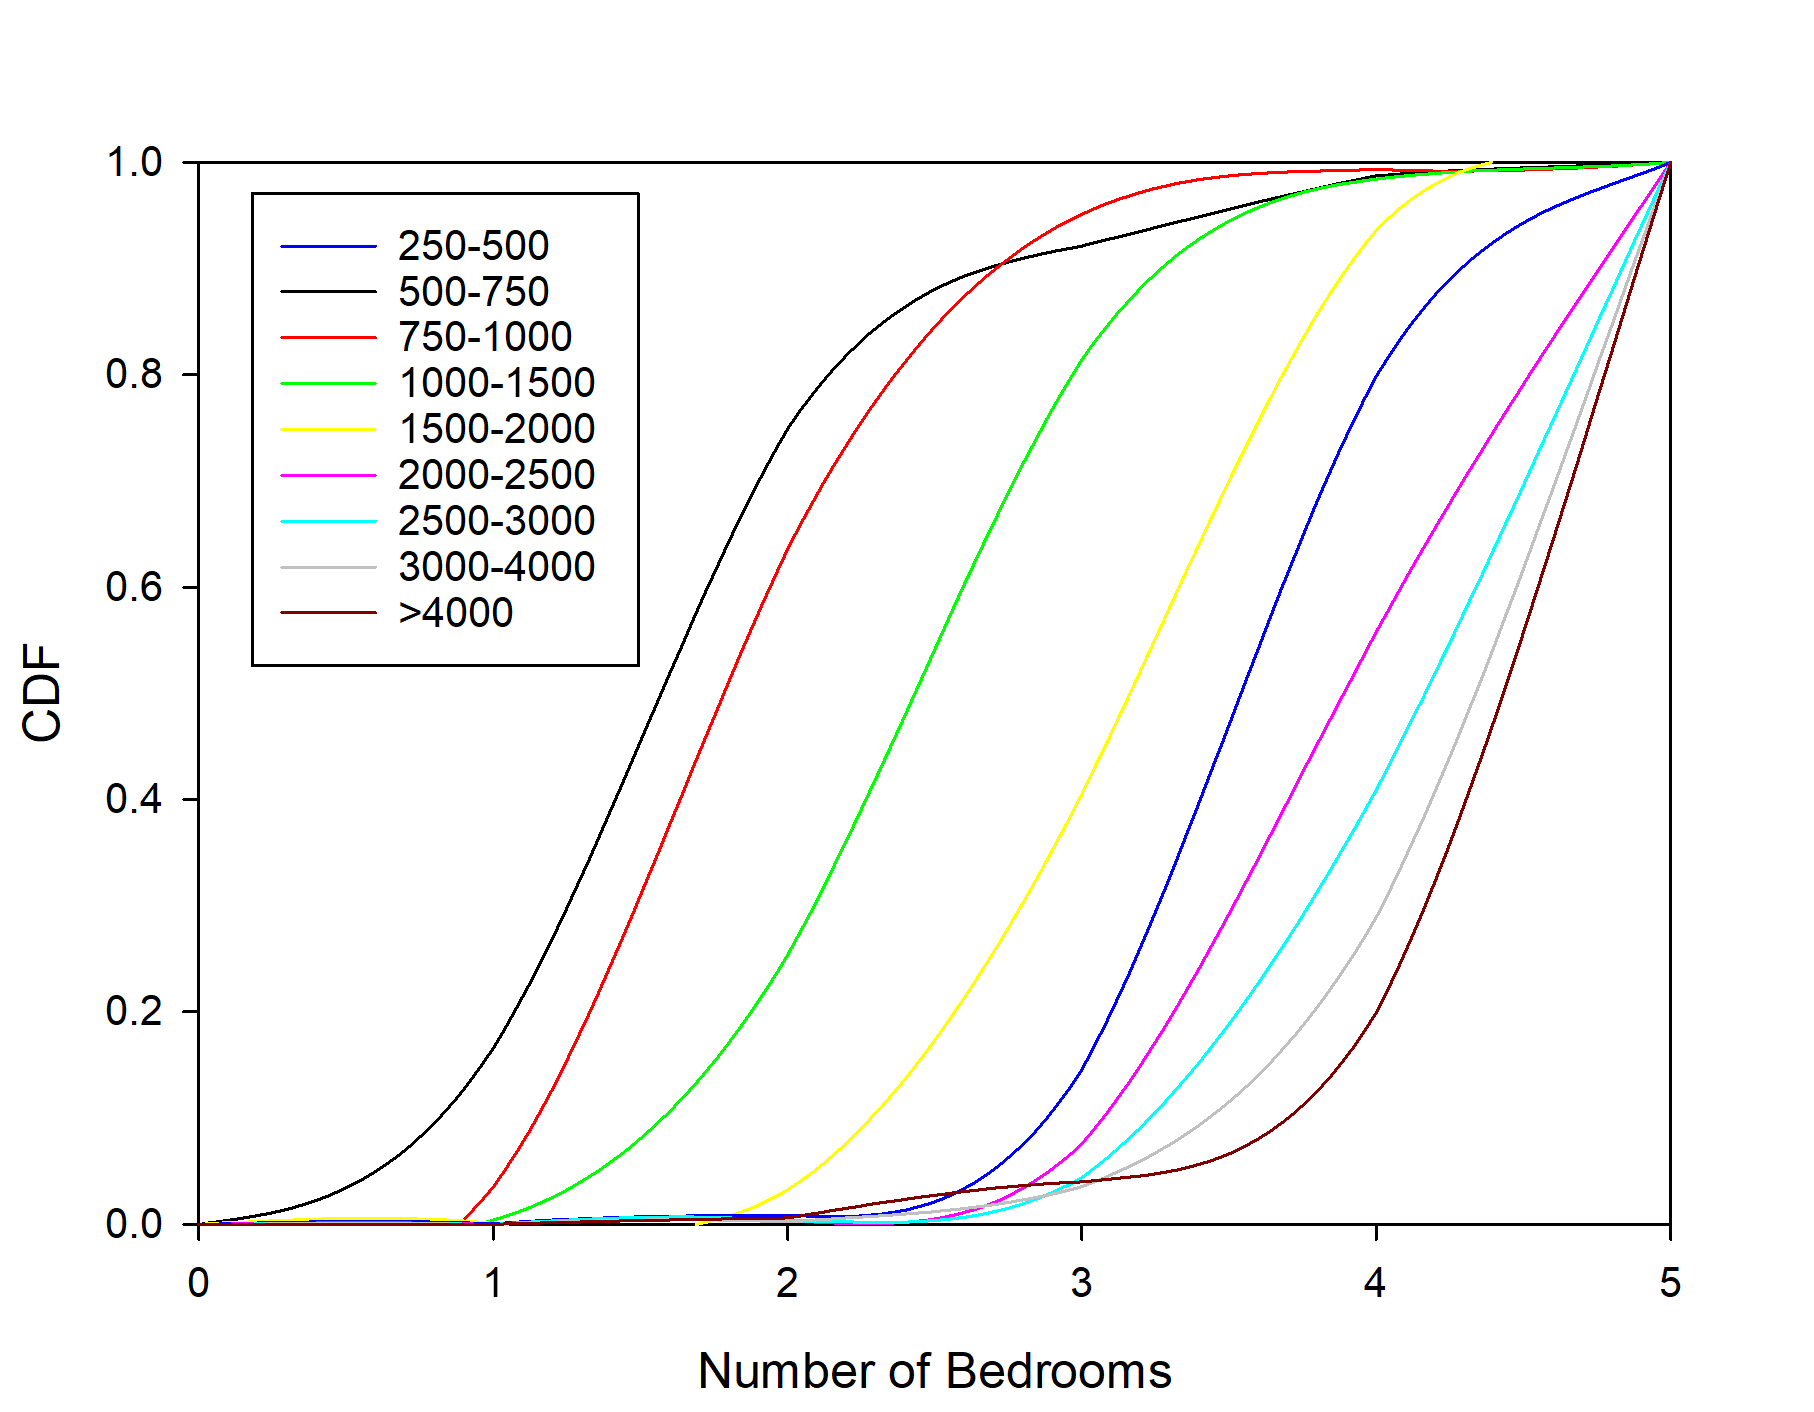
\includegraphics[height=2.5in]{FIGURES/Number_of_Bedrooms} \\
(b) Number of Bedrooms in a Residence as a Function of Total Floor Area \\
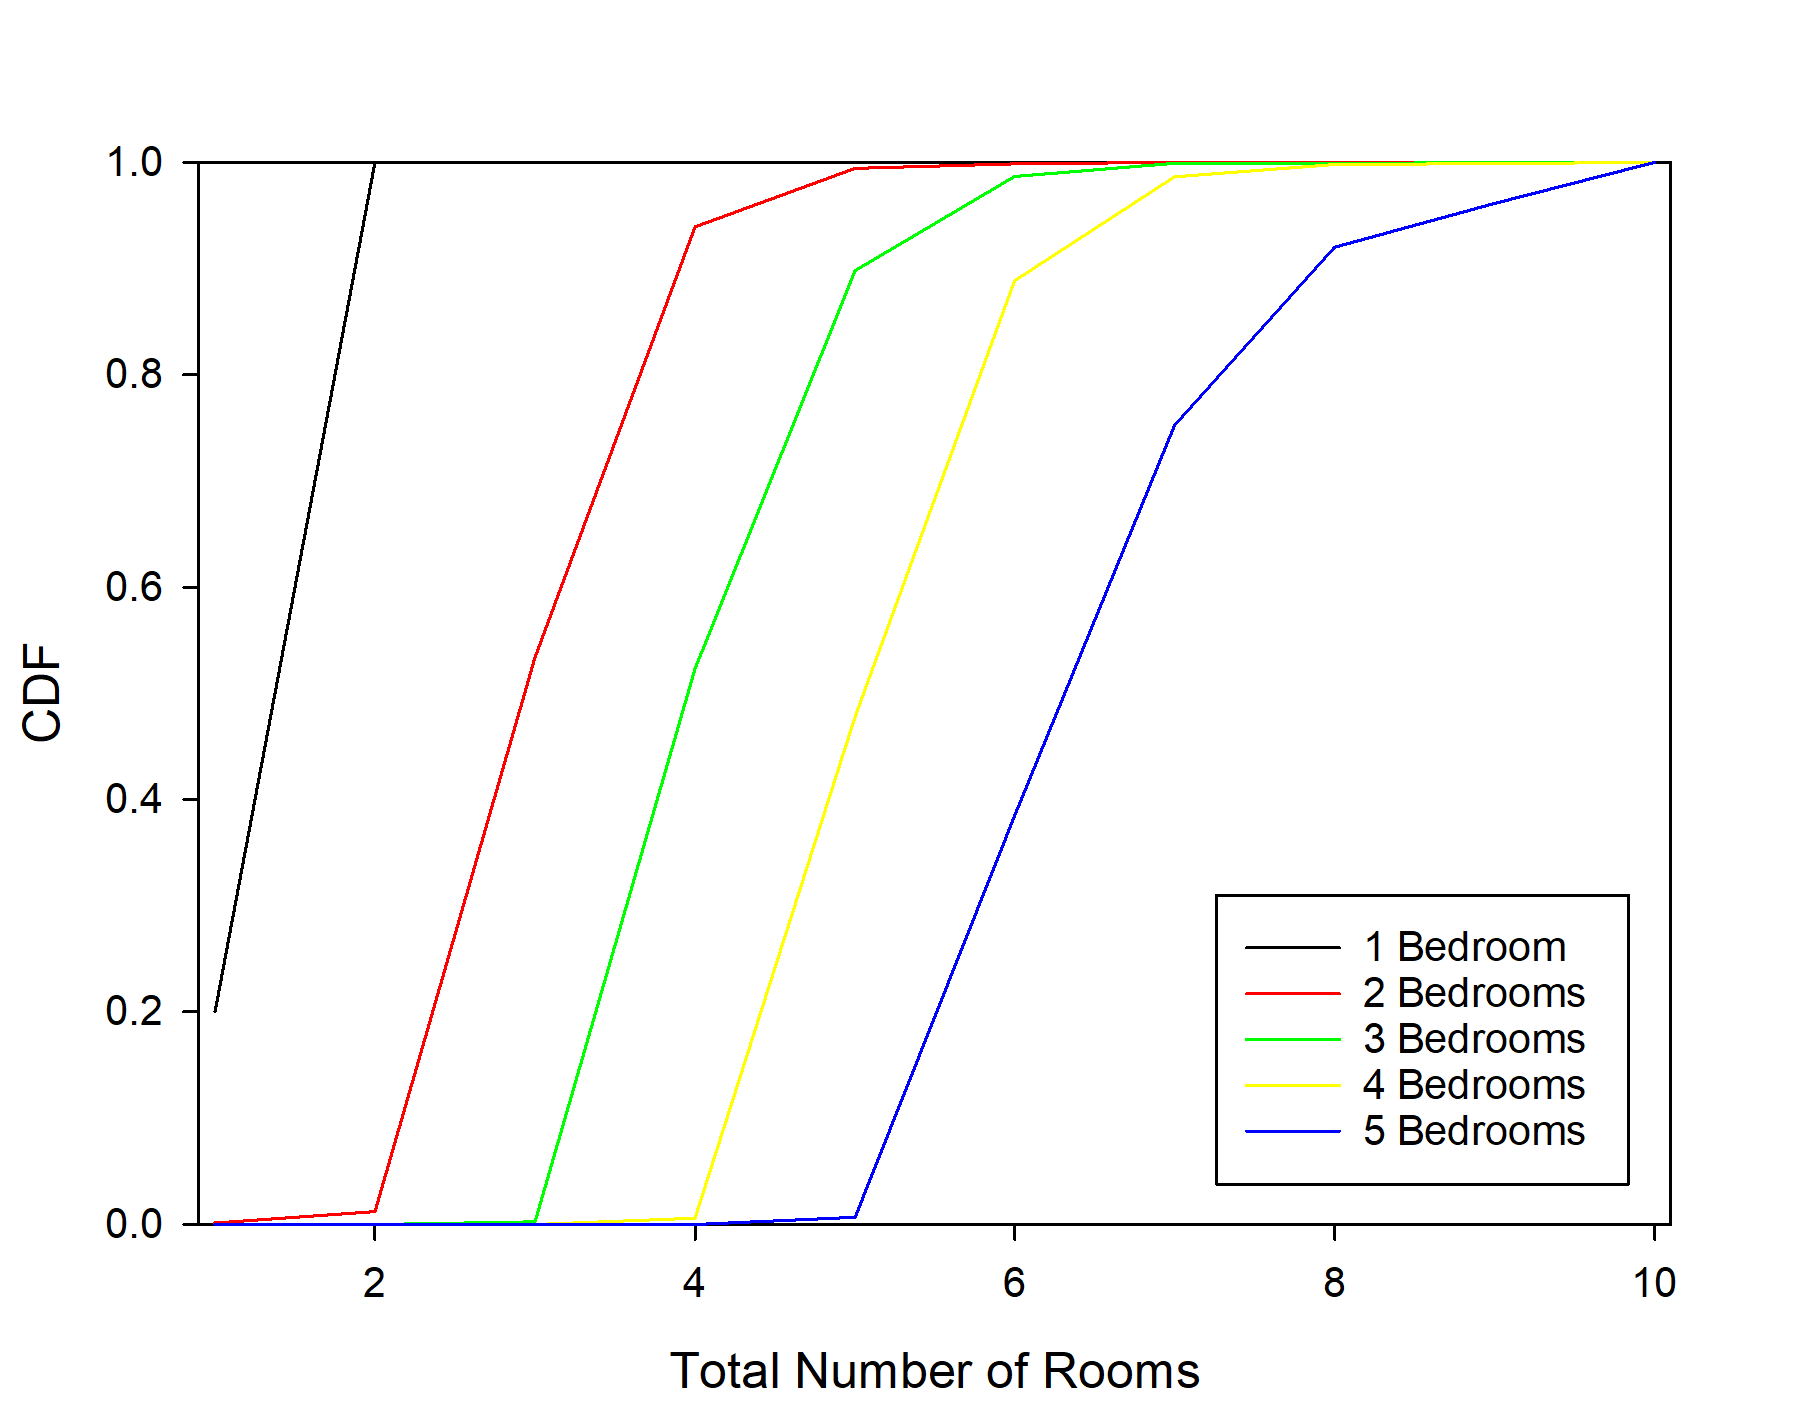
\includegraphics[height=2.5in]{FIGURES/Total_Rooms} \\
(c) Total Number of Rooms as a Function of the Number of Bedrooms in a Residence with  \\
1000 ft$^2$ - 1500 ft$^2$ of Total Floor Area  \\
\end{tabular*}
\caption[Cumulative Probability Distributions for Home Size, Number of Bedrooms and Total Number of Rooms]
{Example Cumulative Probability Distributions for Home Size, Number of Bedrooms and Total Number of Rooms (excluding Bathrooms) taken from the 2015 U.S. Housing Survey \cite{AHS2015}}
\label{sample_room_distribution}
\end{figure}

Other characteristics of the structure such as materials of construction, vent openings, fire definitions, measurement targets, sprinklers, and detection devices can be varied as desired for the problem being studied. Table \ref{tbl:distributable_variables} shows variables in the modeling that can be varied based on user-defined distributions \footnote{The content of this table follows the form of that used in B-Risk \cite{BranzFire}, adapted to be applicable to the calculational capabilities of the CFAST model.}.

\noindent
\begin{longtable}{@{\extracolsep{\fill}}|l|l|l|}
\caption[CFAST Inputs That Can be Varied Based on User-Defined Distributions]{CFAST Inputs That Can be Varied Based on User-Defined Distributions}
\label{tbl:distributable_variables} \\ \hline
\parbox{2in}{\bf Category}    & \parbox{2in}{\bf Input}  & \parbox{2in}{\bf Units} \\ \hline
\endfirsthead
\caption[]{Continued} \\ \hline
\parbox{2in}{\bf Category}    & \parbox{2in}{\bf Input}  & \parbox{2in}{\bf Units} \\ \hline
\endhead
Ambient Conditions      & Interior Temperature          & \degc                     \\
                        & Exterior Temperature          & \degc                     \\
                        & Relative Humidity             & \%                        \\ \hline
Thermal Properties      & Thermal Conductivity          & kW/(m~\degc)              \\
                        & Specific Heat                 & kJ/(kg~\degc)             \\
                        & Density                       & kg/m$^3$                  \\
                        & Default Thickness             & m                         \\
                        & Emissivity                    &                           \\ \hline
Compartments            & Width                         & m                         \\
                        & Depth                         & m                         \\
                        & Height                        & m                         \\
                        & Width Position                & m                         \\
                        & Depth Position                & m                         \\
                        & Height Position               & m                         \\
                        & Wall Leak Area Ratio          & m$^2$/m$^2$               \\
                        & Floor Leak Area Ratio         & m$^2$/m$^2$               \\ \hline
 Wall Vents             & Sill                          & m                         \\
                        & Soffit                        & m                         \\
                        & Width                         & m                         \\
                        & Initial Opening Fraction      & 0-1                       \\
                        & Open/Close Time               & s                         \\
                        & Final Opening Fraction        & 0-1                       \\
                        & Setpoint                      & s, \degc, or kW/m$^2$     \\
                        & Pre-Activation Fraction       & 0-1                       \\
                        & Post-Activation Fraction      & 0-1                       \\ \hline
 Ceiling / Floor Vents  & Cross-Sectional Area          & m$^2$                     \\
                        & Initial Opening Fraction      & 0-1                       \\
                        & Open/Close Time               & s                         \\
                        & Final Opening Fraction        & 0-1                       \\
                        & Setpoint                      & s, \degc, or kW/m$^2$     \\
                        & Pre-Activation Fraction       & 0-1                       \\ \hline
 Mechanical Vents       & From Compartment Area         & m$^2$                     \\
                        & From Compartment Height       & m                         \\
                        & To Compartment Area           & m$^2$                     \\
                        & To Compartment Height         & m                         \\
                        & Flow Rate                     & m$^3$/s                   \\
                        & Begin Dropoff                 & Pa                        \\
                        & End Dropoff                   & Pa                        \\
                        & Initial Opening Fraction      & 0-1                       \\
                        & Open/Close Time               & s                         \\
                        & Final Opening Fraction        & 0-1                       \\
                        & Setpoint                      & s, \degc, or kW/m$^2$     \\
                        & Pre-Activation Fraction       & 0-1                       \\
                        & Post-Activation Fraction      & 0-1                       \\
                        & Filter Efficiency             & \%                        \\
                        & Begin Filtering Time          & s                         \\ \hline
Fires                   & \multicolumn{2}{|c|}{See Section \ref{Fire_Scenarios}}    \\ \hline
Targets                 & Width Target Position         & m                         \\
                        & Depth Target Position         & m                         \\
                        & Height Target Position        & m                         \\
                        & Width Normal Vector           & 0-1                       \\
                        & Depth Normal Vector           & 0-1                       \\
                        & Height Normal Vector          & 0-1                       \\
                        & Target Points To              & Selection List            \\
                        & Thickness                     & m                         \\
                        & Internal Temperature Location & m                         \\ \hline
Detection / Suppression & Width Position                & m                         \\
                        & Depth Position                & m                         \\
                        & Height Position               & m                         \\
                        & Activation Temperature        & \degc                     \\
                        & Activation Obscuration        & \%/m                      \\
                        & RTI                           & (m~s)$^{1/2}$             \\
                        & Spray Density                 & m/s                       \\ \hline
\end{longtable}

\clearpage

\section{Fire Scenarios}
\label{Fire_Scenarios}

\subsection{Individual Variables}

The quantitative definition of fires is arguably the most important \cite{Babrauskas:1992} and complex of all the inputs in any fire modeling scenario. It includes specification of the fire location, fuel composition, ignition criterion, heat release rate, burning area, and species yields, most of which can vary with time over the course of the fire.

\noindent
\begin{longtable}{@{\extracolsep{\fill}}|l|l|l|}
\caption[CFAST Fire Inputs That Can be Varied Based on User-Defined Distributions]{CFAST Fire Inputs That Can be Varied Based on User-Defined Distributions}
\label{tbl:fire_variables} \\ \hline
\parbox{2in}{\bf Category}    & \parbox{2in}{\bf Input}  & \parbox{2in}{\bf Units} \\ \hline
\endfirsthead
\caption[]{Continued} \\ \hline
\parbox{2in}{\bf Category}    & \parbox{2in}{\bf Input}  & \parbox{2in}{\bf Units} \\ \hline
\endhead
Fire Location           & Compartment                   & Selection List                \\
                        & Width Position                & m                             \\
                        & Depth Position                & m                             \\ \hline
Fuel Composition        & Carbon Molecules              & $\geq$ 0                      \\
                        & Hydrogen Molecules            & $\geq$ 0                      \\
                        & Oxygen Molecules              & $\geq$ 0                      \\
                        & Nitrogen Molecules            & $\geq$ 0                      \\
                        & Chlorine Molecules            & $\geq$ 0                      \\
                        & Heat of Combustion            & kJ/kg                         \\
                        & Radiative Fraction            & 0 - 1                         \\ \hline
Ignition Criteria       & Ignition Criterion            & Selection List                \\
                        & Setpoint                      & s, \degc, or kW/m$^2$         \\ \hline
Time Histories          & \multicolumn{2}{|c|}{See Section \ref{Fire_Time_Histories}}   \\ \hline
\end{longtable}

\subsection{Time Histories}
\label{Fire_Time_Histories}

Some examples of different definitions of time histories go here.

\noindent
\begin{longtable}{@{\extracolsep{\fill}}|l|l|l|}
\caption[CFAST Fire Time Histories That Can be Varied Based on One or More User-Defined Distributions]{CFAST Fire Time Histories That Can be Varied Based on One or More User-Defined Distributions}
\label{tbl:fire_variables} \\ \hline
\parbox{2in}{\bf Category}    & \parbox{2in}{\bf Input}  & \parbox{2in}{\bf Units} \\ \hline
\endfirsthead
\caption[]{Continued} \\ \hline
\parbox{2in}{\bf Category}    & \parbox{2in}{\bf Input}  & \parbox{2in}{\bf Units} \\ \hline
\endhead
Time Histories          & HRR                           & kW                        \\
                        & Fire Height                   & m                         \\
                        & Fire Area                     & m$^2$, >0                 \\
                        & CO Yield                      & kg CO/kg fuel             \\
                        & Soot Yield                    & kg Soot/kg fuel           \\
                        & HCN Yield                     & kg HCN/kg fuel            \\ \hline
\end{longtable}

\section{Defining Data for Analysis}

Choosing modeling results for analysis depends on the goals of the hazard analysis and the particular technology under study. In the most general sense, this means understanding what results are indicative of improved fire safety. This is not a cost benefit analysis, which is a superset of this analysis and outside the scope of this project. To improve fire safety generally means reducing the deaths and injuries due to a fire. So, the goal is to identify which variables, that can be calculated, would give an indication that a new technology will reduce deaths and injuries.

\section{Examples}

\subsection{Example 1: Flashover in a compartment}

The occurrence of flashover within a room is of considerable interest since it is perhaps the ultimate signal of untenable conditions within the room of fire origin and a sign of greatly increased risk to other rooms within the building. Many experimental studies of full-scale fires have been performed that quantify the onset of flashover in terms of measurable physical properties. Several approaches have been taken to estimate the onset of flashover within a room. These methods are typically based on simplified mass and energy balances on a single-compartment fire along with correlations to fire experiments. Walton and Thomas \cite{Walton:2016} provide a review of available methods for calculating temperatures in fires in a single compartment with an open door. Three methods are identified from the works of Babrauskas \cite{Babrauskas:1980}, McCaffrey et al. \cite{McCaffrey:1981uq} and Thomas \cite{Thomas:1981fk}. Additional correlations by Babrauskas \cite{Babrauskas:1980} and H\"ugglund \cite{Hagglund:1980} are available. Deal and Beyler \cite{Valid:DealandBeyler} evaluated some of these correlations with a database derived from more than 250 room fire experiments and provided additional guidance for cases involving forced ventilation. This example uses the Monte Carlo capabilities in CData to generate a set of data to compare these correlations to a range of CFAST simulations. Figure \ref{flashover_geometry} shows the compartment geometry for the simulations.

\begin{figure}[h!]
\centering
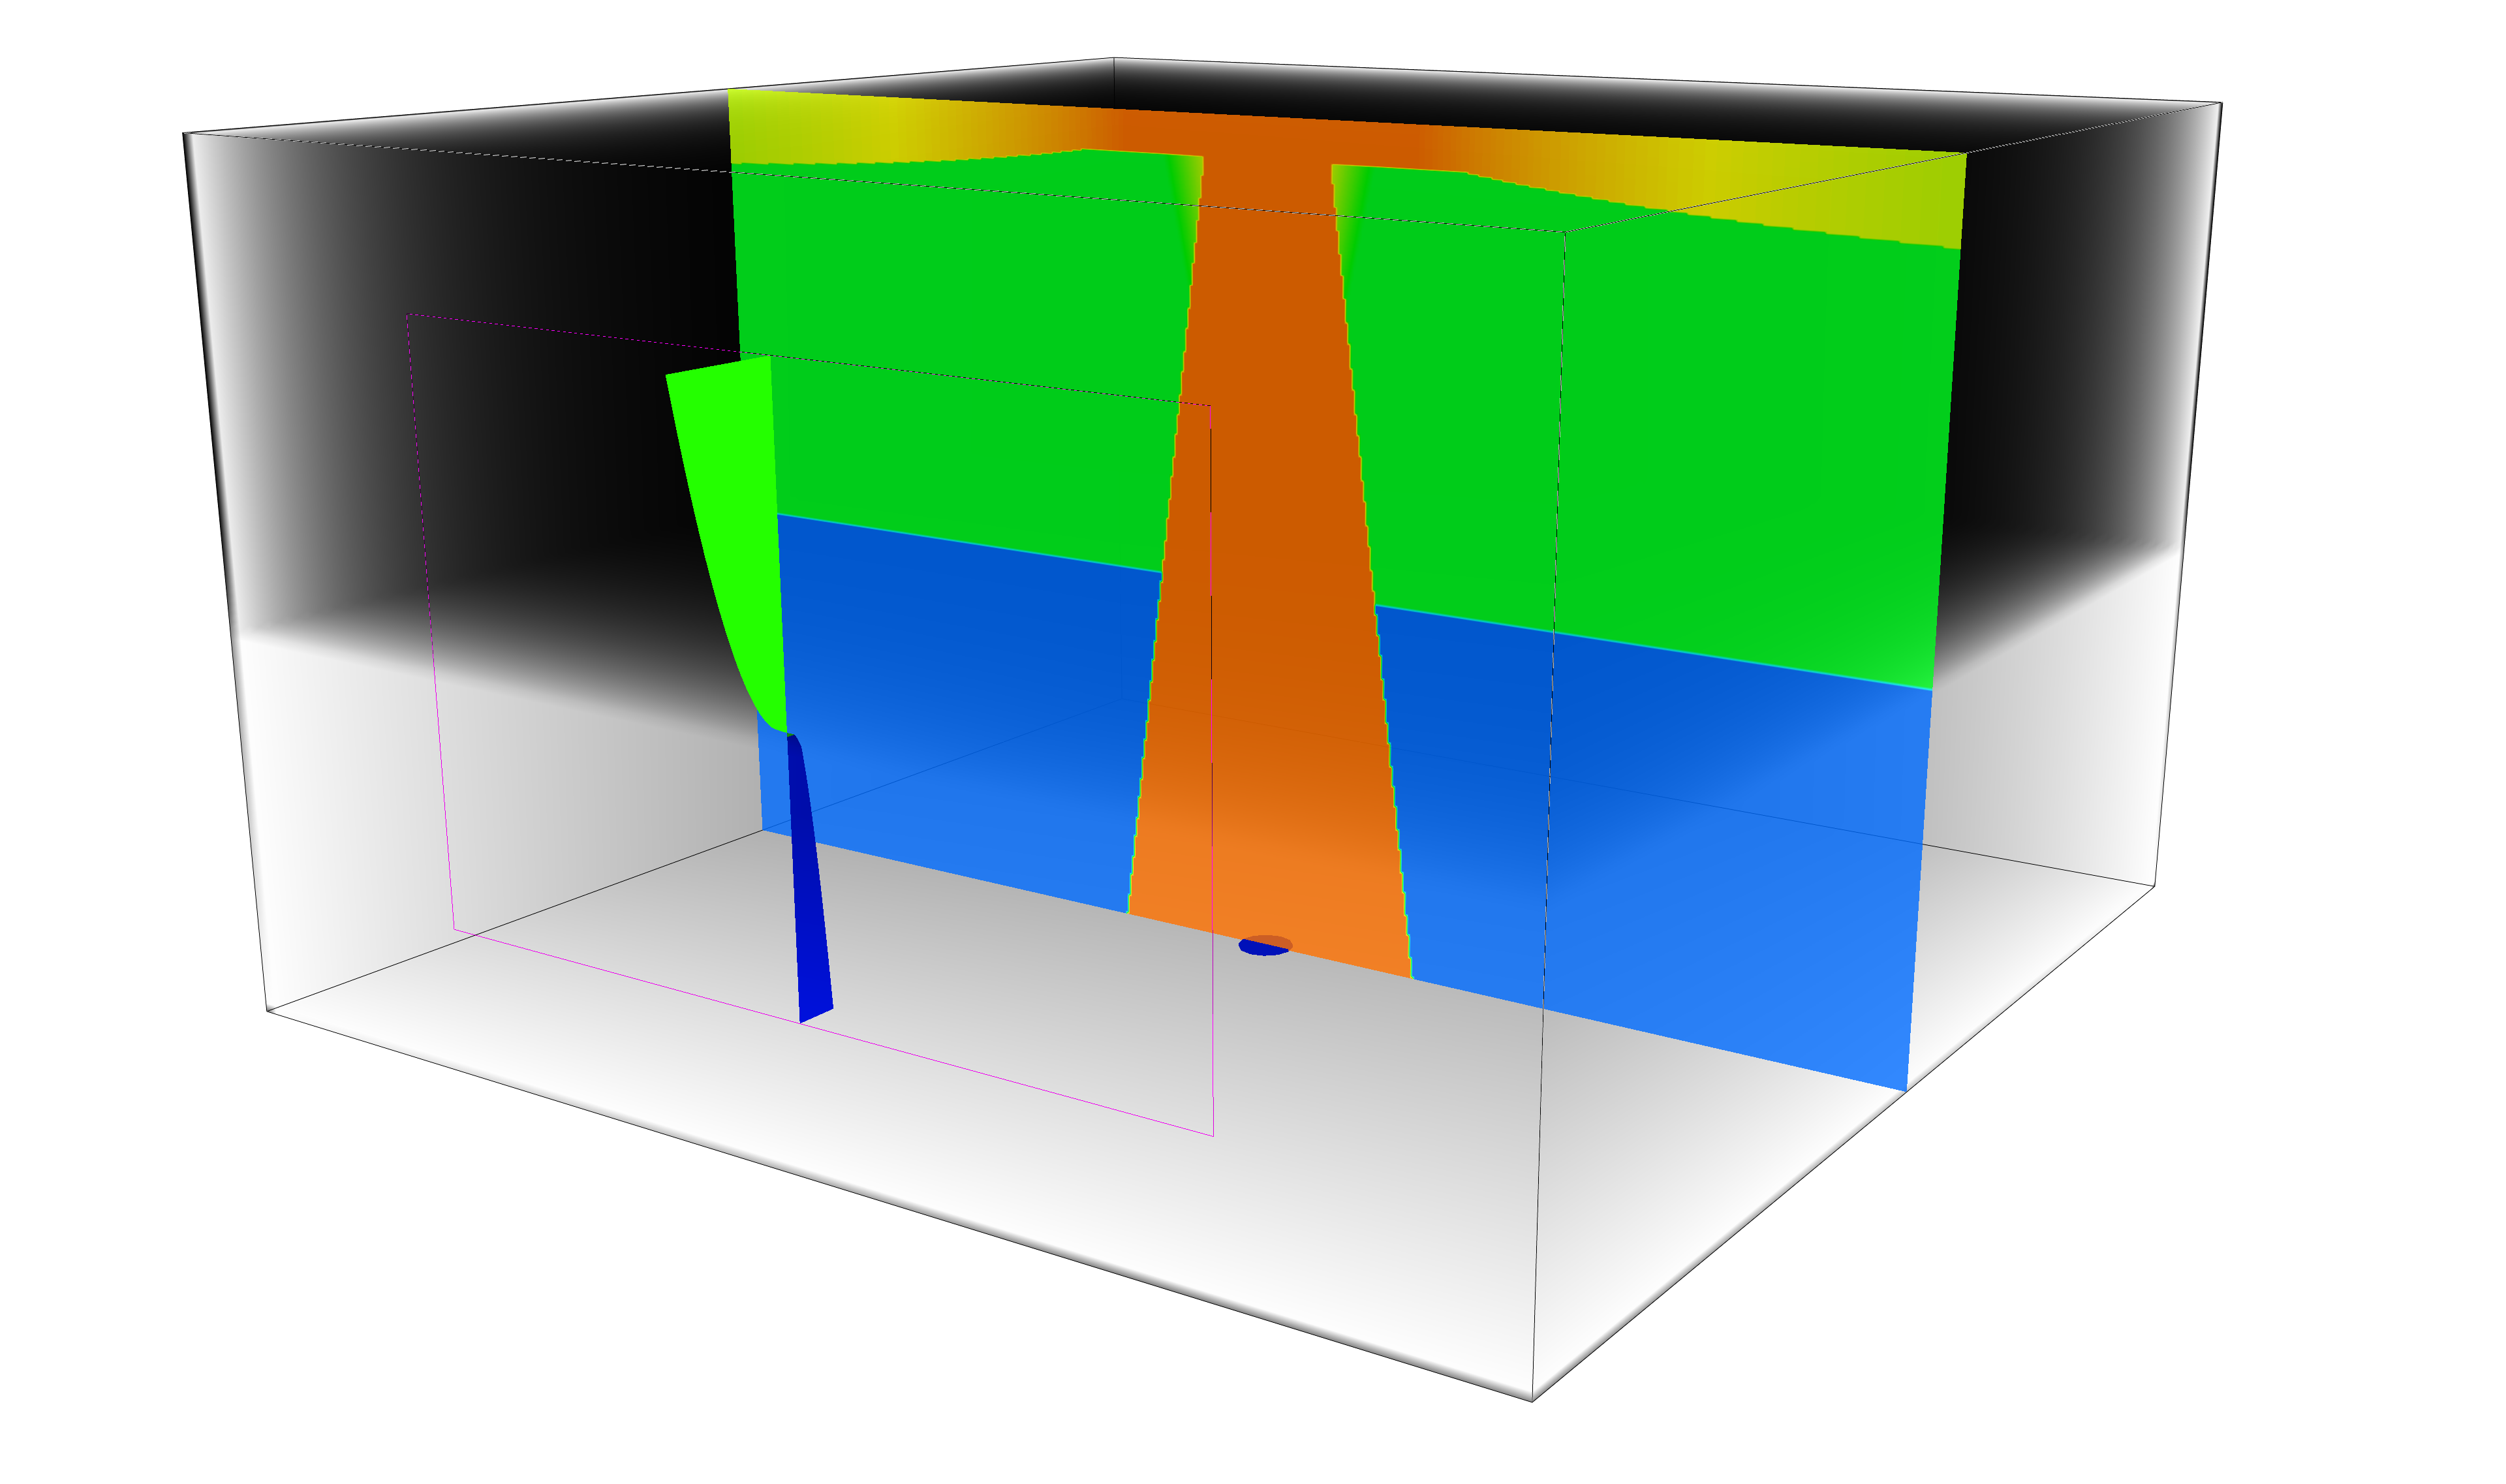
\includegraphics[width=4.5in]{FIGURES/Flashover.png}
\caption{Sample CFAST visualization of a single compartment structure used for example 1.}
\label{flashover_geometry}
\end{figure}

A single compartment with gypsum ceiling and walls and a concrete floor includes a single vent. For this example, the room dimensions, vent dimensions, and fire growth rate are varied as follows:

\begin{description}
\item[Compartment dimensions:] Compartment sizes varied with a uniform distribution scaling all compartment dimensions from 2 m x 2 m x 2 m to 10 m x 10 m x 10 m.
\item[Vent dimensions:] Vent sizes varied with a uniform distribution scaling vent bottom from 0 m to 1.5 m, a uniform distribution scaling vent top from 2 m to 9 m limited by compartment height, and a uniform distribution scaling vent width from 0.25 m to 9 m limited by compartment width.
\item[Fire growth rate:] Fire size varied with a uniform distribution ranging from 75 s to 1 MW to 600 s to 1 MW. Peak heat release rate set to 10 MW to ensure flashover in the compartment when there is sufficient oxygen.
\end{description}

For the analysis, we will look at the minimum heat release rate necessary to achieve flashover in the compartment defined by the typically-used metrics of 600 \degc upper layer temperature and 20~kW/m$^2$ heat flux at floor level \cite{Valid:Peacock_Flashover_1} \cite{Valid:Peacock_Flashover_2}.

\subsection{Example 2: Impact of smoke detector interconnection}

Battery-powered smoke alarms with wireless interconnect signal transmission allow for retrofitting of homes with interconnected smoke alarms up to the current code-required installation locations without hardwiring. However, wireless communication draws additional current beyond basic smoke alarm operation and will affect battery life. To receive an interconnect signal, wireless smoke alarms must periodically power up the transceiver and listen for a transmitted signal from another alarm that initially responds to smoke. Naturally a question arises: what is an acceptable maximum delay time for wireless interconnected smoke alarms given the desire to extend battery life?

In this simplified example based on earlier work \cite{Cleary_2019}, we look at the impact of a periodic activation of wireless communications in detectors. We will use a fixed single-story residential structure for the simulations, varying the fire placement and size, the opening/closing of doors within the structure, and the properties of the smoke detectors placed in each compartment. Figure \ref{detector_geometry} shows the compartment geometry for the simulations.

\begin{figure}[h!]
\centering
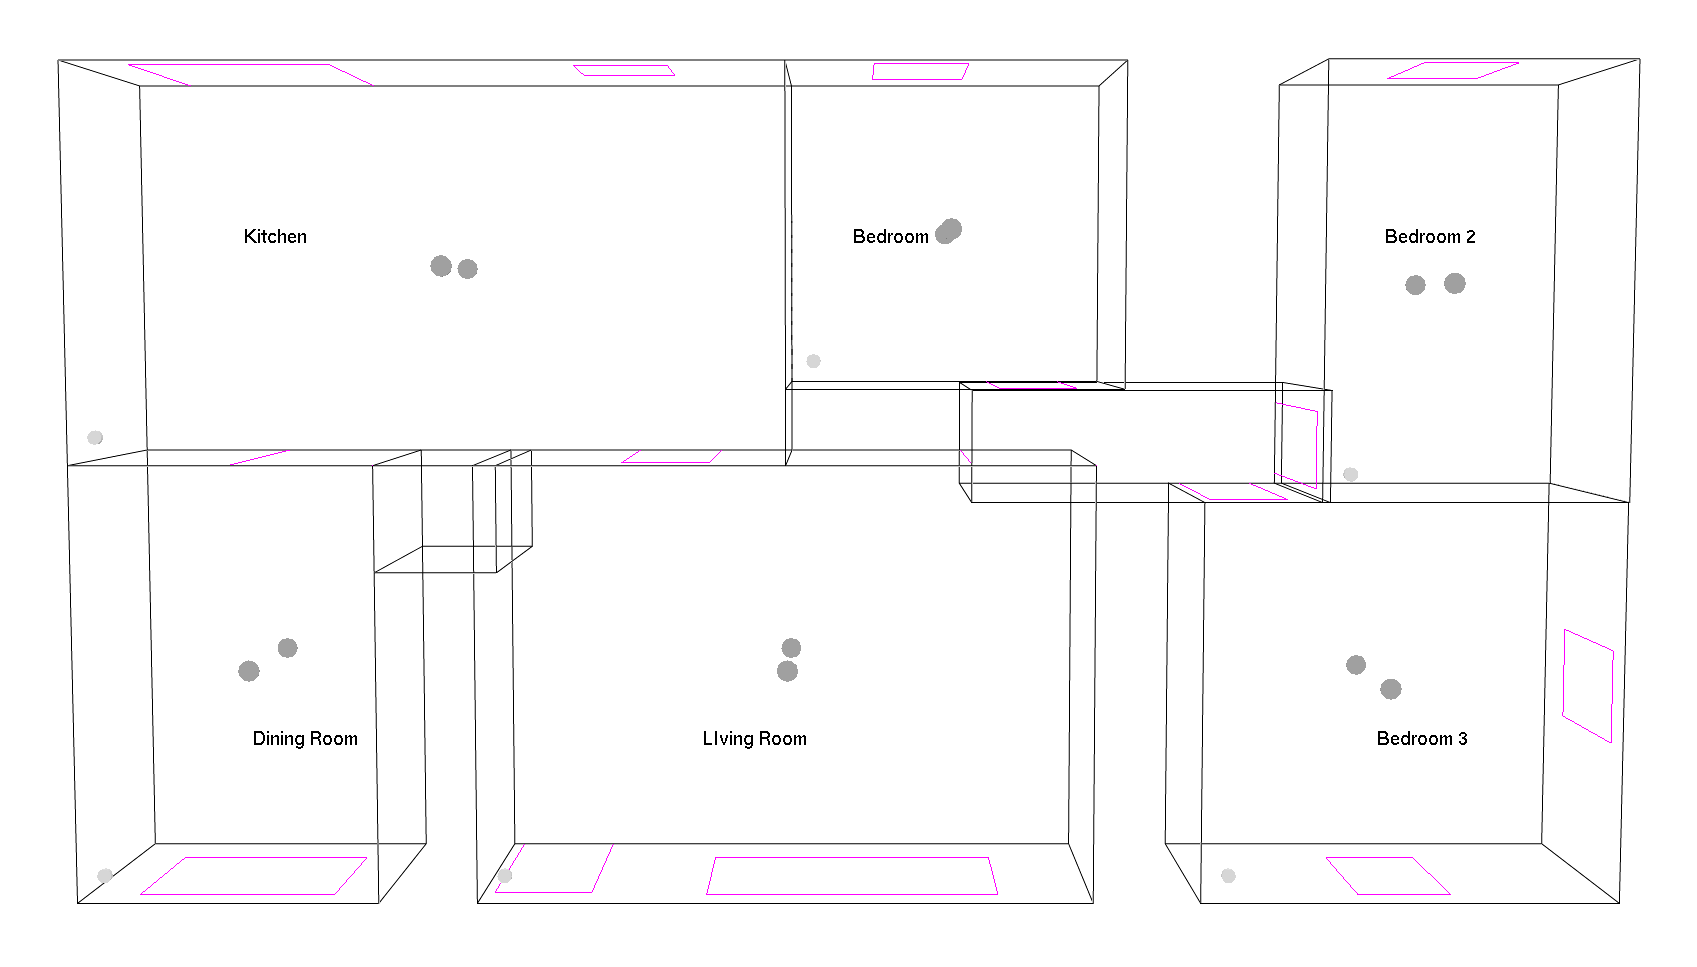
\includegraphics[width=6.5in]{FIGURES/Detectors.png}
\caption{Sample CFAST visualization of a single story residential structure used for example 2.}
\label{detector_geometry}
\end{figure}

For this example, the fire location, fire growth, fire peak heat release rate, vent opening/closing for all interior vents, and smoke detector sensitivity will be varied as follows:

\begin{description}
\item[Fire location:] Fire is placed in a fixed location in a randomly chosen compartment in the structure and is equally split between flaming and smoldering fires.
\item[Initial fire growth rate:] Flaming fires grow from zero to 23~kW $\pm$ 7~kW in 207~s $\pm$ 46~s using normal distributions, followed by a t$^2$ growth to 1054~kW in 222~s $\pm$ 47~s again using a normal distribution. Smoldering fires grow from zero to 11~ kW $\pm$ 3~kW in 6863~s $\pm$ 1812~s using normal distributions, followed by a t$^2$ growth to 1054~kW in 189~s $\pm$ 48~s again using a normal distribution.
\item[Interior doors:] Doors between all interior compartments are each randomly set to be initially fully open or with a 2.5~cm undercut the full width of the door. These openings remain unchanged throughout a simulation.
\item[Smoke detectors:] Smoke detectors follow a statistical smoke alarm activation model developed for upholstered furniture containing polyurethane foam \cite{Cleary:2017}. For this simple example,we use only one detector who activation varies with a log-normal distribution with a geometric mean of 9.5 \%/m $\pm$ 4.2 \%/m (3.0~\%/ft $\pm$ 1.3 \%/ft) for flaming fires and 15.5 \%/m $\pm$ 4.2 \%/m (5.0~\%/ft $\pm$ 1.3 \%/ft) for smoldering fires.
\end{description}

In the analysis, we will look at the impact of delays in triggering of secondary, interconnected smoke detectors on the overall tenability for a range of fires.

\subsection{Example 3: Model Sensitivity}

In this example, we look at a simple fire model sensitivity analysis, which ASTM E 1355 defines as a study of how changes in model parameters affect the results \cite{CFAST:ASTM:E1355}. In other words, sensitivity refers to the rate of change of the model output with respect to input variations. The standard also indicates that model predictions may be sensitive to (1) uncertainties in input data, (2) the level of rigor employed in modeling the relevant physics and chemistry, and (3) the accuracy of numerical treatments. Thus, the purpose of a sensitivity analysis is to assess the extent to which uncertainty in the model inputs is manifested as uncertainty in the model results of interest. For this simple example, we will use a single office building and look at the impact of changing important model inputs by $\pm 10$ \%. Figure \ref{sensitivity_geometry} shows the compartment geometry for the simulations.

\begin{figure}[h!]
\centering
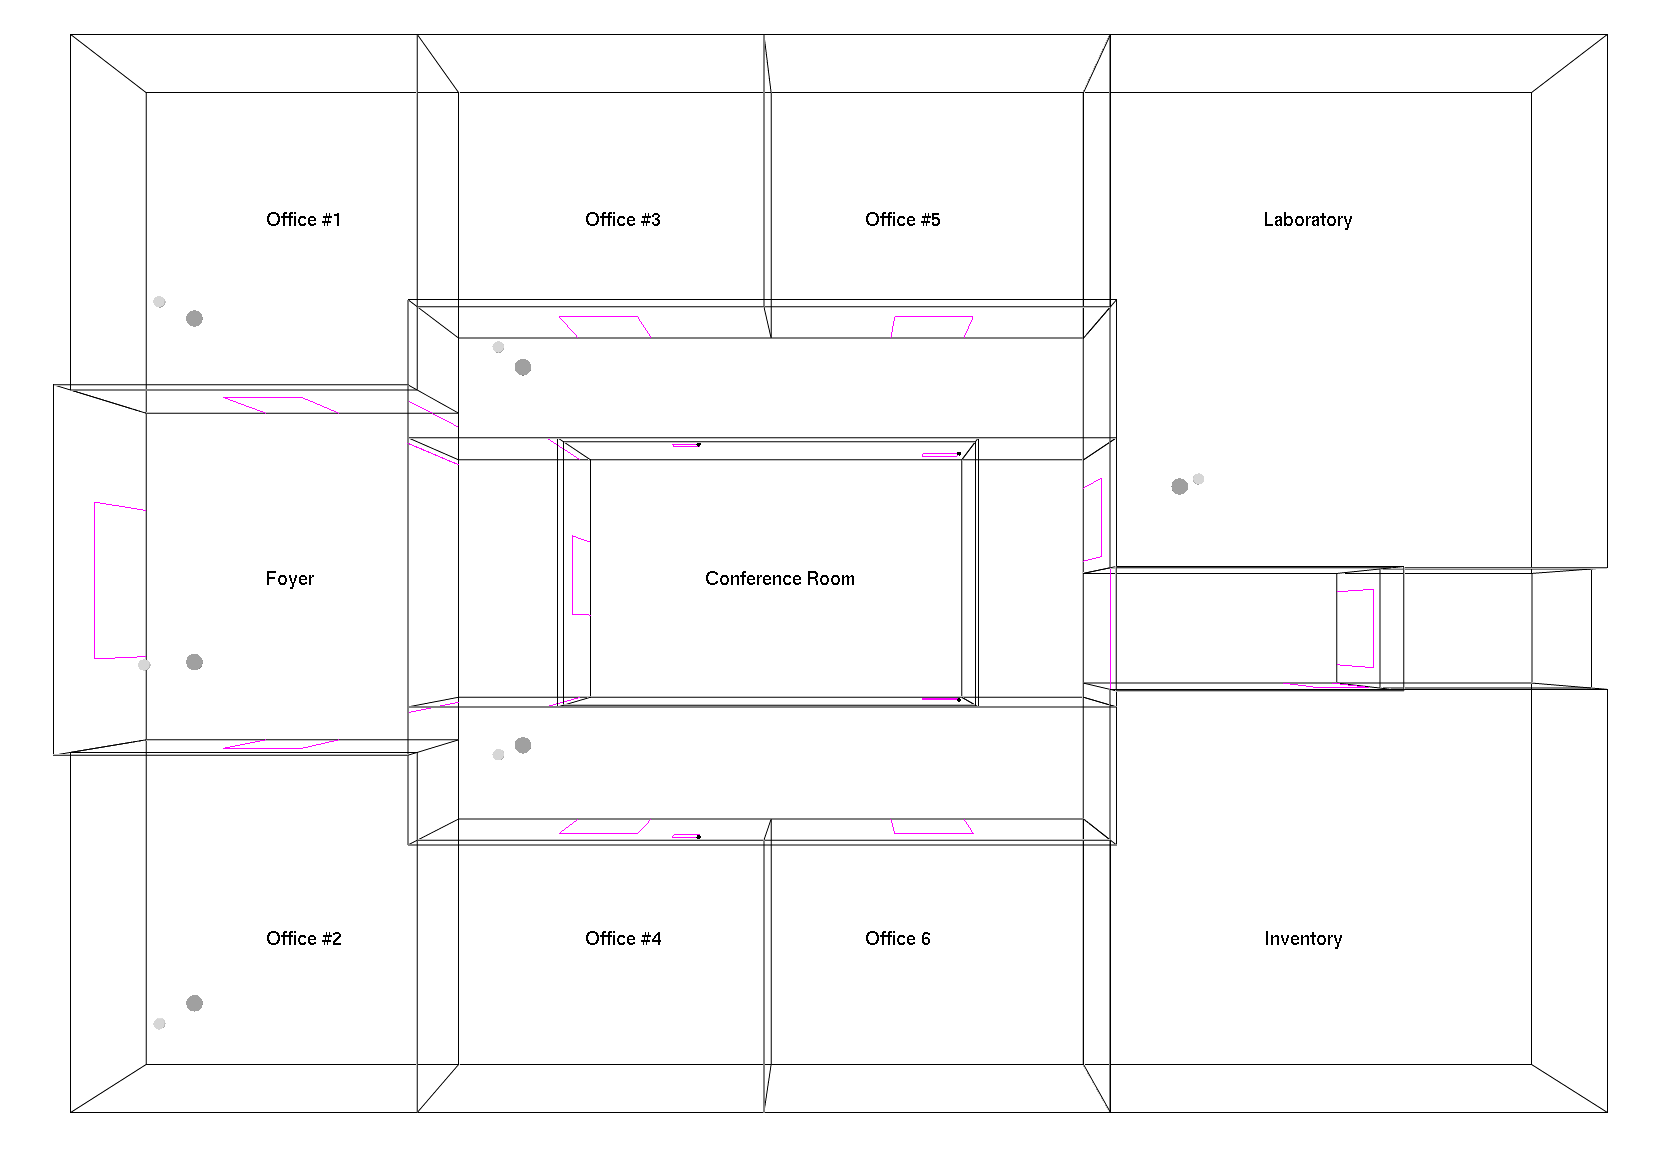
\includegraphics[width=6.5in]{FIGURES/Sensitivity.png}
\caption{Sample CFAST visualization of a single story commercial structure used for example 3.}
\label{sensitivity_geometry}
\end{figure}

A sensitivity analysis involves defining a base case scenario, and varying selected input parameters. The resultant variations in the model output are then measured with respect to the base case scenario, in order to consider the extent to which uncertainty in model inputs influences model output. Therefore, a sensitivity analysis of CFAST should account for variations in the extensive number of input parameters that describe the building geometry, compartment connections, construction materials, and description of one or more fires.

For this example, we will independently vary the following inputs by $\pm$~10~\%, recognizing that these are not an exhaustive list of input variables, but which should represent the major model inputs to a simulation:

\begin{description}
\item[Compartment geometry:] Compartment size will be scaled to $\pm$ 10~\% of base size in all dimensions.
\item[Compartment materials:] Thermal properties for all materials will be varied by $\pm$ 10~\% of base values for thermal conductivity, density, and specific heat. Thickness will be  varied by $\pm$ 10~\% of base values.
\item[Compartment doors:] The size of compartment doors, both interior and exterior, will be  varied by $\pm$ 10~\% of base values for height and width. All interior vents will be open for this example.
\item[Mechanical ventilation:] For mechanical ventilation, the height of each vent, area of each vent, and fan flowrate will each be varied by $\pm$ 10~\% of base values.
\item[Fire:] Fire is in one of the rooms. Peak heat release rate of the fire and time of the peak will be varied by $\pm$ 10~\% of base value. Yields of carbon monoxide and soot will each be varied by $\pm$ 10~\% of base value. Position of the fire is varied by $\pm$ 10~\% of base values in width and depth, and height.
\item[Detectors:] Sensitivity of heat detectors will be varied by $\pm$ 10~\% of base values for activation temperature and RTI. Smoke detector activation obscuration will be varied by $\pm$ 10~\% of base values.
\end{description}

In the analysis, we will look at typically-used outputs to determine those which are more sensitive (a 10 ~\% change in an input value leads to more than a 10~\% change in an output) and less sensitive (a 10 ~\% change in an input value leads to less than a 10~\% change in an output) to a change in selected model inputs to identify the relative importance of selected model inputs to the results of a simulation.

%
%---------------------User's Guide----------------------------------
%

\chapter{Creating Multiple CFAST Runs}
The CData program has several functions. One of them is as a PreProcessor used to create a set of CFAST data files for an analysis. This chapter discusses how the PreProcessor works with some simple examples to demonstrate certain aspects of the system. First is an overview of the basic philosophy behind the PreProcessor. Section \ref{commands_section} discusses all the namelist commands that work in the PreProcessor. The final section discusses the significant issue of storage, which can limit on the size of the analysis that can be done.

\section{Basic Philosophy}

\section{PreProcessor}

\label{commands_section}
Each subsection will discuss one set of namelist inputs and what each of the parameters do. All the inputs are combined in Appendix \ref{preprocessor_reference}  to serve as a reference for commands.

\subsection{Namelist MHDR}

The {\ct \&MHDR} inputs specify details of the scenarios to be generated including the number of cases to be generated, seeds for the random number generator, and locations for input and output files.

\begin{description}
  \item[NUMBER\_OF\_CASES] (default value 1): specifies the number of cases that the preprocessor will generate.
  \item[RANDOM\_SEEDS] (default value, software chosen random integer pair): defines an integer pair used to determine random number seeds for distributions. Any two integers (excluding -1001 which is used internally to indicate default values) may be specified. Including random seeds here will ensure that the same cases will be generated each time the preprocessor is run for a given input file. Changing the random seeds (or other inputs) will result in a different set of input files.  All seeds are written in the {\ct <project>\_seeds.csv} file, if specified.
  \item[WRITE\_RANDOM\_SEEDS] (default value, .TRUE.): if .TRUE., all random number seeds are saved in the file {\ct <project>\_seeds.csv}.
  \item[PARAMETER\_FILE] (default value, {\ct <project>\_parameters.csv} where {\ct <project>} is the base filename of the CDATA/CFAST input file): Summary output file from the preprocessor that list the CFAST file names and parameter values for inputs varied for each CFAST scenario in the set of generated CFAST cases. This file is combined with the summary statistics generated by the accumulator module.
  \item[WORK\_FOLDER] (default value, current folder): folder where the preprocessor creates its set of CFAST inputs file and where the accumulator looks for CFAST output files to be processed.
  \item[OUTPUT\_FOLDER] (default value, current folder): folder where the accumulator or statistics modules put their output files of analysis results.
\end{description}

\vspace{\baselineskip}
\noindent Example:
\begin{lstlisting}
&MHDR NUMBER_OF_CASES = 10000 /
&MHDR NUMBER_OF_CASES = 20000 WRITE_SEEDS = .TRUE.
	PARAMETER_FILE = 'Outputfile' WORK_FOLDER = 'Z:\'  OUTPUT_FOLDER = '..\project'/
\end{lstlisting}



\subsection{Namelist MRND}

The {\ct \&MRND} defines a random number generator that uses a number of inputs to specify distributions for variation. A generator specifies a single random variable for each case so that every input using a particular generator will get the same value for each case. In the simplest cases every field that a user wants to vary will require a separate random generator. However, suppose the desire is to have all the rooms have the same height ceiling, then all the fields will use the same random number generator. % This might be to early to say all this. What do you think?

\begin{description}
  \item[ID] Distributions are defined by a unique alphanumeric name. This may be as simple as a single character or number, or a description of the distribution. All IDs must be unique throughout an input file.
  \item[FYI] A user defined comment that can provide additional information about the input.
  \item[TYPE] identifies the type of distribution. Additional required inputs depend of the type of distribution defined. Allowed distributions are {\ct CONSTANT},  {\ct UNIFORM}, {\ct TRIANGLE}, {\ct NORMAL}, {\ct LOG\_NORMAL}, {\ct BETA}, {\ct LINEAR }, and {\ct USER\_DEFINED}.
  \item[RANDOM\_SEEDS] like {\ct RANDOM\_SEEDS} in {\ct \&MHDR}, an integer pair specifies initial seeds for the random number generator, but applies only to the specific distribution. Any two integers (excluding -1001 which is used internally to indicate default values) may be specified. Including random seeds here will ensure that the same cases will be generated each time the preprocessor is run for a given input file. Changing the random seeds (or other inputs) will result in a different set of input files. All seeds are written in the {\ct <project>\_seeds.csv} file, if specified.
  \item[INTEGER\_VALUES] a set of integer values for the {\ct USER\_DEFINED} distribution type. Values for an individual scenario are chosen randomly from the list of values provided.
  \item[LOGICAL\_VALUES]a set of logical values for the {\ct USER\_DEFINED} distribution type. Values for an individual scenario are chosen randomly from the list of values provided.
  \item[PROBABILITIES] a set of probabilities values for the {\ct USER\_DEFINED} distribution type. These are not cumulative probabilities and the total of all values must add to 1.0
  \item[REAL\_VALUES] a set of real values for the {\ct USER\_DEFINED} distribution type. Values for an individual scenario are chosen randomly from the list of values provided.
  \item[STRING\_VALUES] a set of string values for the {\ct USER\_DEFINED} distribution type. Values for an individual scenario are chosen randomly from the list of values provided.
  \item[CONSTANT] is a constant value. For the {\ct CONSTANT} distribution it is the value that is returned by the generator. 
  \item[MINIMUM] minimum value for the {\ct UNIFORM}, {\ct TRIANGLE}, and {\ct LINEAR} distribution types.
  \item[MAXIMUM] maximum value for the {\ct UNIFORM}, {\ct TRIANGLE}, and {\ct LINEAR} distribution types.
  \item[PEAK] peak value for the {\ct TRIANGLE} distribution type.
  \item[ALPHA] alpha value for the {\ct BETA} distribution type.
  \item[BETA] beta value for the {\ct BETA} distribution type.
  \item[MEAN] mean value for the {\ct NORMAL}; geometric mean value for the {\ct LOG\_NORMAL} distribution type.
  \item[STDEV] standard deviation value for the {\ct NORMAL}; geometric standard deviation value for the {\ct LOG\_NORMAL} distribution type.
  \item[MINIMUM\_FIELD] specifies the name of the specific input (i.e., the name of a compartment, vent, etc.) and the specific field within that input that is to be taken as the minimum value of the distribution returned. It allows the range to be defined by another input. For example, if the {\ct \&MRND} input is used to vary the ceiling height the top of a vent can be used as the lowest value for the ceiling height by including a {\ct MINIMUM\_FIELD} input for the compartment height input such as {\ct MINIMUM\_FIELD="Vent 1", "TOP"} to limit how low height of the compartment is set.
  \item[MAXIMUM\_FIELD] specifies the name of the specific input (i.e., the name of a compartment, vent, etc.) and the specific field within that input that is to be taken as the maximum value of the distribution returned. It allows the range to be defined by another input. For example, if the {\ct \&MRND} input is used to vary the top of a vent, then you can set the upper limit the height in the associated compartment by including a {\ct MAXIMUM\_FIELD} input for the vent input such as {\ct MAXIMUM\_FIELD="Comp 1","HEIGHT"} to cap the vent top to the height of the compartment.
\end{description}

\vspace{\baselineskip}
\noindent Example:
\begin{lstlisting}
&MRND ID = 'Example rand generator', TYPE = 'UNIFORM',  MINIMUM = 10, MAXIMUM = 50 /
&MRND ID ='Second rand generator', TYPE = 'NORMAL', MEAN = 0, STDEV = 1 /
\end{lstlisting}

\subsection{Namelist MFLD}

\begin{description}
  \item[ID] Varied input fields are defined by a unique alphanumeric name. This may be as simple as a single character or number, or a description of the field. All IDs must be unique throughout an input file.
  \item[FYI] A user defined comment that can provide additional information about the input.
  \item[FIELD] specifies the name of the specific input (i.e., the name of a compartment, vent, etc.) and the specific field within that input that is to be varied. For example, {\ct FIELD="Comp 1","HEIGHT"} would vary the height of the compartment named {\ct Comp 1}.
  \item[TYPE] specifies the type of field data used to fill in values in the specified field. Additional inputs depend on the type of field specified. Allowed field types are {\ct VALUE}, {\ct SCALING}, {\ct LABEL}, and {\ct INDEX}. {\ct VALUE} simply takes the value returned from the specified random generator and places it directly in the specified field. {\ct SCALING} takes the returned value and multiplies by the {\ct BASE\_SCALING\_VALUE} and puts that value in the field. {\ct INDEX} requires the random generator to return integers as an index into the {\ct VALUES} input (starting at 1 to the number of inputs in the {\ct VALUES}       input for the current {\ct \&MFLD} input). The value in the {\ct INDEX\_TYPE}, {\ct REAL}, {\ct INTEGER}, {\ct CHARACTER}, or {\ct LOGICAL}, array at the index is placed in the field.
  \item[FIELD\_LABELS] The purpose of this optional is simply to provide descriptions of the purpose of each index value for {\ct INDEX} inputs.
  \item[RAND\_ID] specifies the ID of associated {\ct \&MRND} input used to provide random inputs for the field. These may be unique to each field input or more than one field input may use the same {\ct \&MRND} input to coordinate values for multiple input fields. The number of inputs in the {\ct \&MRND} input must match those for the field type.
  \item[ADD\_TO\_PARAMETERS] set to .TRUE. to include the value of the field in the parameters file, {\ct <project>\_parameters.csv}. Default value is .TRUE.
  \item[PARAMETER\_COLUMN\_LABEL] specifies the column title for this input field in the parameters file, {\ct <project>\_parameters.csv}. If it is not included CData will use a combination of the {\ct FIELD} inputs to create a column label.
  \item[VALUES] a set of values for the {\ct INDEX} field type. Values for an individual scenario are chosen randomly from the list of values provided. The type of the inputs is by the type of value needed from the {\ct FIELD} input but all inputs in the {\ct VALUES} inputs are specified in a character array input.
  \item[BASE\_SCALING\_VALUE] Initial value of the field for the {\ct SCALING} type field. Defaults to the value in the base input file if not included.
\end{description}

\vspace{\baselineskip}
\noindent Example:
\begin{lstlisting}
&MFLD ID = 'Height_bedroom' FIELD = 'Bedroom', 'HEIGHT' RAND_ID = 'uniform_generator' PARAMETER_COLUMN_LABEL = 'Bedroom height' /
\end{lstlisting}

\clearpage

\subsection{Namelist MFIR}

\begin{description}
  \item[ID]
  \item[FYI]
  \item[FIRE\_ID] This is the fire in the data file that you are modifying. Everything in a single namelist will modify this fire. 
  \item[BASE\_FIRE\_ID] If you are doing scaling a fire this is the fire that will be used. Basically, this is the place that the base values are stored. In the future there might even be a list of fires that could be copied into this fire.\ 
  \item[MODIFY\_FIRE\_AREA\_TO\_MATCH\_HRR] This hasn’t been implemented yet. It is going to be a real valued variable. If it is negative, then the fire areas are not modified. If it has a positive value, the fire area is modified using Kevin’s equation with the value in the variable. We should put some limits on the values they can put here. Probably fairly close to 1. 
  \item[SCALING\_FIRE\_HRR\_RANDOM\_GENERATOR\_ID] A scaling value that is applied to all the HRR values in a fire. This is done before the Incipient fire model is calculated so it won’t impact the delay or HRR value for the initial fire.
  \item[SCALING\_FIRE\_TIME\_RANDOM\_GENERATOR\_ID] A scaling value that is applied to all the TIME values in a fire. This is done before the Incipient fire model is calculated so it won’t impact the delay or HRR value A scaling value that is applied to all the HRR values in a fire. This is done before the Incipient fire model is calculated so it won’t impact the delay or HRR value for the initial fire. 
  \item[ADD\_HRR\_SCALE\_TO\_PARAMETERS] Defaults to {\ct .TRUE.}
  \item[HRR\_SCALE\_HEADER] If left blank will be filled in by the code.
  \item[ADD\_TIME\_SCALE\_TO\_PARAMETERS] Defaults to {\ct .TRUE.}
  \item[TIME\_SCALE\_HEADER]
  \item[FIRE\_COMPARTMENT\_RANDOM\_GENERATOR\_ID] A random generator that returns an index to pick which compartment the fire is in. Usually uses USER\_DEFINED\_DISCRETE\_DISTRIBUITION
  \item[FIRE\_COMPARTMENT\_IDS] A list of compartment names that have a chance of having the fire in them.
  \item[ADD\_FIRE\_COMPARTMENT\_ID\_TO\_PARAMETERS] Defaults to {\ct .TRUE.}
  \item[FIRE\_COMPARTMENT\_ID\_HEADER] 
  \item[FLAMING\_SMOLDERING\_IGNITION\_DELAY\_RANDOM\_GENERATOR\_ID] This and the next two sets of two entries work together. This one determines if you have a Smoldering or Flaming incipient fire. Ignition is not delayed, that is badly worded. If this one is not defined then only one of the two sets of two can be defined and the other two must not be left blank. This is a I{\ct INDEX} type of field because this gives the most flexability
  \item[INCIPIENT\_FIRE\_TYPES] A list made up of 'FLAMING' and 'SMOLDERING'. This allows users to coordinate the incipeint begining of the fire with other inputs in the scenario.
  \item[TYPE\_OF\_INCIPIENT\_GROWTH] Probably can go away but was easier to include in the begining. Defaults to {\ct NONE} but can be {\ct FLAMING}, {\ct SMOLDERING}, and {\ct RANDOM}
  \item[FLAMING\_IGNITION\_DELAY\_RANDOM\_GENERATOR\_ID] This is the first of the flaming set of generators. Both must be defined. If you don’t want the value to change you can set it up to a {\ct CONSTANT} random generator. This one determines how long the incipient flaming fire burns.
  \item[PEAK\_FLAMING\_IGNITION\_RANDOM\_GENERATOR\_ID] God these names are awful. This one determines the final HRR for the flaming fire ramp. It is important to understand that using this means the first two HRR points will be overwritten and all times for all entries in the fire will be set to the same.
  \item[SMOLDERING\_IGNITION\_DELAY\_RANDOM\_GENERATOR\_ID] This is the smoldering pair that match the above.
  \item[PEAK\_SMOLDERING\_IGNITION\_RANDOM\_GENERATOR\_ID] Same as above for smoldering fire.
  \item[ADD\_IGNITION\_TYPE\_TO\_PARAMETERS] Defaults to {\ct .TRUE.} Displays 'FLAMING' or 'SMOLDERING' depending on which type of ignition happens. 
  \item[ADD\_SMOLDERING\_IGNITION\_TIME\_TO\_PARAMETERS] Defaults to {\ct .TRUE.}
  \item[ADD\_SMOLDER\_IGNTION\_PEAK\_TO\_PARAMETERS] Name shortened becasue adding the 'ING' made the variable name too long and it got truncated. Defaults to {\ct .TRUE.}
  \item[ADD\_FLAMING\_IGNTION\_TIME\_TO\_PARAMETERS] Defaults to {\ct .TRUE.}
  \item[ADD\_FLAMING\_IGNITION\_PEAK\_HRR\_TO\_PARAMETERS] Defaults to {\ct .TRUE.}
  \item[FLAMING\_HRR\_PEAK\_HEADER]  
  \item[FLAMING\_TIME\_HEADER]
  \item[SMOLDERING\_HRR\_PEAK\_HEADER]
  \item[SMOLDERING\_TIME\_HEADER]
  \item[FIRE\_TIME\_GENERATORS] The following group probably should best be explained in a call. It isn't that complicate but I don't think I would get it correct in text. 
  \item[FIRE\_HRR\_GENERATORS]
  \item[NUMBER\_OF\_GROWTH\_POINTS]
  \item[NUMBER\_OF\_DECAY\_POINTS]
  \item[GROWTH\_EXPONENT]
  \item[DECAY\_EXPONENT]
  \item[ADD\_HRR\_TO\_PARAMETERS]
  \item[ADD\_TIME\_TO\_PARAMETERS]
  \item[HRR\_LABELS]
  \item[TIME\_LABELS]
\end{description}

\subsection{Namelist DUMP}

\begin{description}
  \item[ID] Summary outputs are defined by a unique alphanumeric name. This may be as simple as a single character or number, or a description of the output. All IDs must be unique throughout an input file.
  \item[FYI] A user defined comment that can provide additional information about the input.
  \item[FILE] specifies which of the CFAST output files are used for the summary output. Allowable inputs are {\ct COMPARTMENTS}, {\ct DEVICES}, {\ct FIRES}, {\ct MASSES}, or {\ct WALLS}.
  \item[TYPE] specifies the type of summary data to calculate. Allowable input are {\ct MIN}, {\ct MAX}, {\ct TRIGGER\_LESSER}, {\ct TRIGGER\_GREATER}, {\ct INTEGRATE}, {\ct TOTAL\_HRR}. For {\ct MIN} or {\ct MAX}, only the {\ct FIRST\_FIELD} input is required. For {\ct TRIGGER\_LESSER} or {\ct TRIGGER\_GREATER}, the value the of first device when the second device passes the value in {\ct CRITERION}. For {\ct INTEGRATE}, {\ct FIRST\_FIELD} must be {\ct "Time", "Simulation Time"}. {\ct INTEGRATE} integrates the values of {\ct SECOND\_FIELD} over the entire simulation time.
  \item[FIRST\_FIELD] specifies the name of the specific input (i.e., the name of a compartment, vent, etc.) and the specific field within that input that is to be used for the first input in a calculation. For example, {\ct FIELD="Time","Simulation Time"} would specify the simulation time.
  \item[SECOND\_FIELD] specifies the name of the specific input (i.e., the name of a compartment, vent, etc.) and the specific field within that input that is to be used for the second input in a calculation, if required. For example, {\ct FIELD="Comp 1","Upper Layer Temperature"} would specify the upper layer temperature in compartment named {\ct Comp 1}.
  \item[CRITERION] Specifies the value to be evaluated in a {\ct TRIGGER\_LESSER} or {\ct TRIGGER\_GREATER} calculation.
\end{description}

\vspace{\baselineskip}
\noindent Example:
\begin{lstlisting}
&DUMP ID = 'Total Time Completed'
     FILE_TYPE = 'DEVICES'  TYPE = 'MAXIMUM'
     FIRST_FIELD = 'Time', 'Simulation Time' /
&DUMP ID = 'Fire Room Ion Detector'
     FILE = 'DEVICES'  TYPE = 'TRIGGER_GREATER'  CRITERIA = 1
     FIRST_FIELD = 'Time', 'Simulation Time'
     SECOND_FIELD = 'Ionization Detector Room 1', 'Sensor Activation' /
\end{lstlisting}

\clearpage

\section{Running CFAST}

\subsection{Running on Different Operating Systems}

\subsection{The Question of Storage}

\section{Generating Statistics}

\subsection{Accumulator}

\subsection{Statistics}

\subsubsection{Determining If Enough Runs Have Been Made}

Monte Carlo analysis is fundamentally grounded in The Law of Large Numbers. The Law of Large Numbers states that for a large-enough number of independent samples, the average converges to the expected value. For example, if we want to know what the probability of flashover is in the kitchen for a certain class of fires, the Law of Large Numbers assures us that the percentage of Monte Carlo runs where flashover occurs converges to the probability as the number of runs becomes large.

The problem here is determining how many runs is enough. Put differently, how many runs does it take to guarantee a result that is "close enough" to be usable? Two strategies are used here. The first is graphing the evolution of the mean versus number of runs. The second is to graph the standard deviation of the mean versus the number of runs. The first strategy should show decreasing variation as the number of runs increases and should converge on a point. The second strategy should show the variance decreasing with the number of runs and approaching zero. The determination of whether the estimates are "close enough" is a judgment of the analyst and will depend on how much accuracy is needed.

\subsubsection{Histograms}

In some cases what is of interest is the distribution of values. There are two approaches to evaluating that  included here. First is a histogram, where the data are sorted into a set of equal bins, and the number of elements in each bin is displayed on a chart. The number of bins used here is automatically selected using Sturges rule \cite{Sturges_1926} which chooses the number of bins according to the rule: \[k = \lceil \log_2 n \rceil + 1\], where  \[ \lceil \rceil\] represents the ceiling function.

\subsubsection{Empirical Probability Density Function}

The post-processor is also capable of generating an empirical probability density function. It does so using the techniques of Kernal Density Estimation \cite{Haste_2009}. To determine the probability density at a point \textit{x} it associates a weight with each point in the data set. The weight is a function of the distance between the point in the data set and \textit{x}. The probability density is then the sum of those weights.

Typically the Gaussian function is used as the Kernal (i.e., the weighting function), although other Kernals are also commonly used. For the Gaussian Kernal (which is used here) the estimated probability density at a point \textit{x} is:

\[f(x) = \frac{1}{Nb}\sum_{j=1}^{N} \phi\left(\frac{x - x_j}{b} \right) \]

where \textit{N} is the number of data points, \[x_j\] is an individual data point, \[\phi\] is the standard normal density function, and \textit{b} is the "bandwidth." The bandwidth determines the width of the window within which the data points contribute significantly to the density estimate. In this implementation, the bandwidth is determined automatically.

\subsubsection{Decision Trees}

Sometimes what is of interest is the relationship one variable has to other variables in the output. There are many ways of estimating relationships, but one of the most intuitive is that of Decision Trees. The approach implemented here is closely related to that of Classification and Regression Trees \cite{Haste_2009}. The output of the algorithm is a binary tree. Each node splits the data into two, until the tree arrives at the leaf nodes. For classification trees, each leaf node is associated with the best-fit category. For regression trees, each leaf node is associated with the average of the data that arrives at that node.

Decision trees have the advantage of being very easy to interpret. Their interpretability is one reason for their popularity. Trees have a couple of drawbacks as well. The most noticable is that their predictions are not smooth. In addition, trees can be highly unstable. That is, small changes in the data can produce large changes in the estimated tree. In addition, there are cases the same data can be represented by very different trees.


%
%-------------------------Analysis of Data-------------------------------------------
%

\chapter{Analysis of Data}

\section{General Analysis (possibly to be removed)}

\section{Examples}

\subsection{Example 1}

\subsection{Example 2}

\subsection{Example 3}

%
% -------------------  Summary ------------------------
%

\chapter{Summary and Future Work}

\bibliography{../Bibliography/CFAST_refs}

\appendix
\addcontentsline{toc}{chapter}{Appendices}

%
% -------------------  Nomenclature ------------------------
%

\chapter{Nomenclature}
\label{nomenclature}

Note that the units associated with a given symbol are sometimes changed upon input to and output from the program. In particular, temperatures are typically input in degrees Celsius, converted to Kelvin, and then converted back to Celsius on output. Energy units involving Joules or Watts are typically input as kJ or kW, converted to J or W, then converted back to kJ or kW.

\begin{center}
\begin{longtable}{p{1in}  p{5.5 in}}

$A$                 & area, m$^2$ \\
\end{longtable}

\end{center}

\chapter{PreProcessor Reference}
\label{preprocessor_reference}
Each subsection will discuss one namelist and what each of the parameters does. The tables presented in each subsection are combined in Appendix XXX  to serve as a refence for commands.

\section{Namelist DUMP}

\section{Namelist MHDR}

\section{Namelist MRND}

\section{Namelist MFLD}

\section{Namelist MFIR}

\section {Namelist MSTT}
\chapter{Supplemental Material}

\chapter{Change Log}

\label{last_page}

\end{document}
